\documentclass{article} % For LaTeX2e
\usepackage{iclr2027_conference,times}
% T1 encoding is needed for accented author names in the bibliography (e.g., \k{e})
\usepackage[T1]{fontenc}

% Line numbers on the left are required by the ICLR submission style (reviewers cite them)
% and disappear automatically under \iclrfinalcopy. To hide them temporarily while editing,
% uncomment the next line, and remember to comment it out again before submission.
% \renewcommand{\iclrruler}[1]{}

\usepackage{amsmath,amssymb,amsthm,mathtools,bm}
\usepackage{booktabs}
\usepackage{multirow}
\usepackage{graphicx}
\usepackage{xcolor}
\usepackage{float}
\usepackage{algorithm}
\usepackage[noend]{algpseudocode}
% Appendix floats use [!htbp] so that LaTeX fills pages itself; \FloatBarrier at section boundaries
% keeps floats from drifting into the next section and avoids the blank pages caused by [H]
\usepackage[section]{placeins}
\renewcommand{\bottomfraction}{0.8}
\renewcommand{\floatpagefraction}{0.85}
\setcounter{topnumber}{4}
\setcounter{bottomnumber}{3}
\setcounter{totalnumber}{6}
% Stack floats from the top of float pages instead of spreading them out vertically
\makeatletter
\setlength{\@fptop}{0pt}
\setlength{\@fpsep}{\floatsep}
\setlength{\@fpbot}{0pt plus 1fil}
\makeatother

% hyperref must come after float-related packages to avoid duplicate anchors
\usepackage{hyperref}
\usepackage{url}

% -------- theorem environments --------
\theoremstyle{plain}
\newtheorem{theorem}{Theorem}[section]
\newtheorem{lemma}[theorem]{Lemma}
\newtheorem{corollary}[theorem]{Corollary}
\newtheorem{proposition}[theorem]{Proposition}
\theoremstyle{remark}
\newtheorem{remark}[theorem]{Remark}

% -------- notation --------
\newcommand{\Expl}{\mathrm{Expl}}
\newcommand{\Proj}{\Pi}
\newcommand{\simplex}{\Delta}
% Vectors are bold lowercase
\newcommand{\bx}{{\bm{x}}}
\newcommand{\by}{{\bm{y}}}
\newcommand{\bv}{{\bm{v}}}
\newcommand{\bw}{{\bm{w}}}
\newcommand{\bz}{{\bm{z}}}
\newcommand{\bu}{{\bm{u}}}
\newcommand{\bd}{{\bm{d}}}
\newcommand{\bq}{{\bm{q}}}
\newcommand{\br}{{\bm{r}}}
\newcommand{\be}{{\bm{e}}}
\newcommand{\brho}{{\bm{\rho}}}
\newcommand{\bell}{{\bm{\ell}}}
\newcommand{\aug}{\tilde{\bell}}
\newcommand{\dx}{\Delta\bx}
\newcommand{\coda}{CoDA}
\newcommand{\codar}{CoDA-R}
\newcommand{\rnad}{R-NaD-PPO}

\title{Coupled Dual-Adversarial Regularized Self-Play}

% Authors must not appear in the submitted version. They are hidden
% as long as the \iclrfinalcopy macro below remains commented out.
\author{Antiquus S.~Hippocampus, Natalia Cerebro \& Amelie P. Amygdale \\
Department of Computer Science\\
Cranberry-Lemon University\\
Pittsburgh, PA 15213, USA \\
\texttt{\{hippo,brain,jen\}@cs.cranberry-lemon.edu}
}

%\iclrfinalcopy % Uncomment for camera-ready version, but NOT for submission.
\begin{document}

\maketitle

\begin{abstract}
Naive self-play for two-player zero-sum games can cycle in nontransitive games. Regularized self-play stabilizes training with a single network but only plays against itself, so it forgets earlier opponents and cannot use external ones; population methods keep an opponent pool, but their equilibrium lives in a mixture over the pool, and heuristic weightings such as PFSP carry no convergence guarantee. We propose Coupled Dual-Adversarial Regularized self-play (CoDA-R). Each round, CoDA-R sets the pool weights by a Euclidean projection anchored at pure self-play, so that only opponents currently beating the latest policy receive weight, and then takes a proximal policy step against the resulting mixture. The coupling yields one energy inequality that charges every policy step and every unit of pool weight to the remaining distance to a Nash equilibrium. For the exact algorithm, this gives last-iterate convergence of the latest policy to a Nash equilibrium however oracle opponents enter or leave the pool, plus certificates computable during training and error-tolerant versions of all bounds. In OpenSpiel at a matched budget, the latest network of CoDA-R cuts the tail exploitability on Goofspiel(4) from 0.797 for R-NaD-PPO to 0.083, on par with a multi-network PSRO mixture; on Leduc poker, with the dual strength scaled to the payoff range and an exact best-response oracle, it roughly halves that of R-NaD-PPO; on Liar's Dice the two tie.
\end{abstract}

% ----------------------------------------------------------------------
\section{Introduction}
% ----------------------------------------------------------------------

Two-player zero-sum games are the most basic model of adversarial decision making. Board games, poker, and real-time strategy games are its most direct instances~\citep{silver2018alphazero,brown2018libratus,vinyals2019alphastar,perolat2022stratego}, and the training objectives of generative adversarial networks and robust optimization can also be written as min--max problems~\citep{goodfellow2014gan,daskalakis2018optimism}. The natural target is a Nash strategy, commonly obtained by self-play, in which the current policy plays against itself or its past versions and is updated by reinforcement learning, requiring neither human data nor explicit opponent modeling.

However, self-play has a well-known failure mode. Real games commonly contain nontransitive components~\citep{czarnecki2020spinning}, and naive self-play, which updates only against the current strongest opponent, spins around in rock--paper--scissors-style cycles and fails to converge~\citep{balduzzi2018mechanics,balduzzi2019openended}. The two families of remedies each leave something to be desired. Regularized self-play (R-NaD, MMD) adds a periodically moving anchor in payoff or policy space, which turns the cyclic dynamics into a contraction toward a regularized equilibrium, with the guarantee landing on a single network~\citep{perolat2021rnad,perolat2022stratego,sokota2023mmd}. The price is that it only plays against itself, so scripted opponents, exploiters trained to counter the current policy, and historical snapshots cannot be plugged in, vulnerabilities off the training trajectory are neither found nor repaired, and earlier strategies are easily forgotten~\citep{openai2019dota,bansal2018emergent}. Population methods (Double Oracle, PSRO, PFSP, and league training) retain historical opponents~\citep{mcmahan2003doubleoracle,lanctot2017psro,vinyals2019alphastar}, but their equilibrium is a mixture over the pool or a separately learned average network, and the network being trained carries no guarantee itself. Heuristic weightings that allocate sampling proportions by win rate or cumulative score (PFSP, the OpenAI Five sampler) almost all lack convergence proofs.

We propose Coupled Dual-Adversarial Regularized self-play (\codar{}), whose pool weights are a dual variable that plays against the current policy (hereafter \emph{latest}), and whose two updates are coupled into an energy inequality that deducts both the movement of latest and the weight held by the pool from the squared distance from latest to a Nash equilibrium (\S\ref{sec:alg}). Since this distance is finite, both must vanish, and a policy that no longer moves while the pool holds no weight can only be a Nash strategy of the full game, however imperfect the exploiter and however the pool changes. This targets settings that neither family covers, for example black-box opponents available only through play (scripted bots, exploiters, legacy agents of other architectures), games too long or costly to evaluate a large pool exhaustively, a pool that changes online, and a single deployed network. PSRO needs the full $N\times N$ meta-game payoff matrix and deploys a mixture, whereas \codar{} needs only the $N$ loss rates of latest, estimated from its own training games; R-NaD-style methods cannot use such opponents, and PFSP uses them without a guarantee. Our novelty lies in the dual rule, which anchors the pool weights at pure self-play and thereby lets an open pool coexist with last-iterate convergence of one network.

\codar{} grew out of an internal predecessor, \coda{}, whose dual anchor moves with training and which converges at rate $O(1/K)$ in the restricted game defined by the pool (\S\ref{sec:coda}). Once the oracle misses a vulnerability, however, latest may stop at a best response to the pool that outside opponents easily beat. Adding latest itself to the pool seems to patch this, but weight then flows to this member with constant loss rate $\tfrac12$ and the moving anchor retains it, pinning latest at a non-Nash point (Proposition~\ref{prop:rps}). \codar{} moves the moving anchor to the primal side and fixes the dual anchor at pure self-play; the energy inequality above comes from this swap. Our contributions are as follows.
\begin{itemize}
\item \textbf{Algorithm.} To our knowledge, \codar{} is the first self-play method that accepts arbitrary external opponents (scripted agents, exploiters, historical snapshots) while guaranteeing that the trained policy itself converges to a Nash equilibrium in the last iterate (exact updates, normal-form games). Prior pool methods guarantee only a mixture or a time average, and regularized self-play admits no external opponents. It needs only game outcomes against each opponent, so any agent that can play may join the pool, and it wraps an unmodified PPO learner up to a proximal reward term (\S\ref{sec:alg}).
\item \textbf{Theory.} A single energy inequality (Theorem~\ref{thm:energy}) charges both policy movement and pool weight to the distance to a Nash equilibrium, so the pool can hold weight only by buying progress toward it. This yields last-iterate convergence of the trained policy, with an explicit $O(K^{-1/4})$ last-iterate rate once the pool stops changing, together with online certificates and error-tolerant versions, for any sequence of pool admissions and any oracle (\S\ref{sec:theory}).
\item \textbf{Experiments.} No inequality is violated in about 3.7 million per-step finite-dimensional records. On OpenSpiel at a matched budget, the single latest network of \codar{} cuts the tail exploitability of \rnad{} on Goofspiel(4) nearly tenfold on all 4 seeds, matching a multi-network PSRO mixture, and roughly halves it on Leduc with an exact best-response (BR) oracle; we also report when the gains depend on oracle strength and payoff scale (\S\ref{sec:exp}).
\end{itemize}

% ----------------------------------------------------------------------
\section{Related Work and Preliminaries}
\label{sec:prelim}
% ----------------------------------------------------------------------

\subsection{Related Work}
\label{sec:related}

\textbf{Population methods.} Double Oracle and PSRO~\citep{mcmahan2003doubleoracle,lanctot2017psro,muller2020generalized,mcaleer2020pipeline} solve a meta-game externally~\citep{wellman2006egta}, PFSP and league training~\citep{vinyals2019alphastar} allocate sampling proportions by win rate, and NFSP~\citep{heinrich2015fsp,heinrich2016nfsp} learns the historical average strategy with a separate network; all of them deploy a mixture of checkpoints or the average network.

\textbf{Regularized self-play.} R-NaD and MMD~\citep{perolat2021rnad,perolat2022stratego,sokota2023mmd} use an anchor in payoff or policy space that moves periodically or is annealed, and optimistic and extragradient methods~\citep{daskalakis2018optimism,mertikopoulos2019omd,nemirovski2004prox,cen2021extragradient} stabilize similarly with an extrapolation term; both are explicit approximations~\citep{mokhtari2020ppa} of the proximal point method~\citep{rockafellar1976ppa}. They guarantee a single network but train only along the self-play trajectory, which is why OpenAI Five and AlphaStar also keep historical opponents~\citep{openai2019dota,vinyals2019alphastar,czarnecki2020spinning}.

\textbf{Multiplicative weights and sleeper members.} The meta-solvers of the PSRO family (Hedge, projected replicator dynamics, MWU) and the opponent sampler of OpenAI Five mostly use multiplicative weights~\citep{lanctot2017psro,mcaleer2022anytime,dinh2022odo,openai2019dota,freund1999hedge}, which accumulate history, so after a member has been suppressed for $T$ rounds, even if it starts countering latest again, it has to win for roughly another $T$ rounds to regain its weight. We call this the \emph{sleeper} problem, which Fixed Share-type algorithms in online learning address~\citep{herbster1998tracking}. Conversely, tied members keep positive weight indefinitely. Methods that deploy the time average are unaffected, but the last iterate of multiplicative weights does not converge in zero-sum games in the first place~\citep{bailey2018mwu}, and members that tie without dropping to zero can further pin latest at a non-Nash point (Proposition~\ref{prop:rps}). We believe this is an important reason why existing pool methods cannot combine a convergence proof with single-network convergence. \codar{} therefore uses a stateless projection (Appendix Table~\ref{tab:related} compares methods).

\subsection{Preliminaries}

Unless otherwise stated, $\|\cdot\|$ denotes the Euclidean ($L_2$) norm throughout.

Consider a finite zero-sum game in which seats are assigned at random in each game, so that the game is symmetric for the two players. A player has $M$ pure strategies, and the mixed strategy space is $X=\simplex_M$. A sequential game can be unfolded over its pure strategies into this form; the theoretical analysis is carried out at this idealized level, and the gap between it and the neural implementation is absorbed into the error terms of \S\ref{sec:inexact}. Let $\ell(\bx;\by)\in[0,1]$ denote the expected loss rate of policy $\bx$ against $\by$. Symmetry gives $\ell(\bx;\by)+\ell(\by;\bx)=1$, so there exists a skew-symmetric matrix $S=-S^\top$ such that
\[
\ell(\bx;\by)=\tfrac12+\bx^\top S\by,\qquad \bx^\top S\bx=0 .
\]
For a frozen opponent $\by_i$, write $\ell_i(\bx):=\ell(\bx;\by_i)$, which is an affine function of $\bx$ with constant gradient $S\by_i$. Policy quality is measured by exploitability,
\[
\Expl(\bx):=\max_{\by\in X}\ell(\bx;\by)-\tfrac12=\max_j(S^\top \bx)_j\ \ge\ 0 .
\]
A Nash strategy satisfies $\Expl(\bx_N)=0$ and exists by the minimax theorem~\citep{vonneumann1928}; moreover,
\begin{equation}
\bx_N\ \text{is Nash}\iff \bx_N^\top S\by\le0\ \ \forall \by\in X\iff \by^\top S\bx_N\ge0\ \ \forall \by\in X .
\label{eq:nash}
\end{equation}
$\Proj_C$ denotes the Euclidean projection onto a closed convex set $C$. Throughout the paper we repeatedly use the variational characterization of the projection (hereafter the obtuse-angle principle)
\begin{equation}
\bw=\Proj_C(\bv)\iff(\bv-\bw)^\top(\bu-\bw)\le0\quad\forall \bu\in C ,
\label{eq:obtuse}
\end{equation}
and the monotonicity and nonexpansiveness it implies~\citep{bauschke2011convex}. The diameter of the simplex is $D=\sqrt2$. Projection onto the simplex takes an $O(N\log N)$ thresholding algorithm, and components below the threshold are exactly zero~\citep{duchi2008projection}.

% ----------------------------------------------------------------------
\section{\coda{}: A Moving Dual Anchor in the Restricted Game}
\label{sec:coda}
% ----------------------------------------------------------------------

\coda{} solves a \emph{restricted game}. Fix an opponent pool $P=\{\by_1,\dots,\by_N\}$ and write $\bell(\bx):=(\ell_1(\bx),\dots,\ell_N(\bx))$. The restricted game between the pool and latest is $\min_{\bx\in X}\max_{\brho\in\simplex_N}\brho^\top\bell(\bx)$, whose value is denoted $v^*$. The dual function $\varphi(\brho):=\min_\bx\brho^\top\bell(\bx)$ is concave, and $v^*=\max_\brho\varphi(\brho)$. One step of \coda{} is parameterized by a dual anchor $\brho_k\in\simplex_N$ and computes the regularized saddle point
\begin{equation}
(\bx_{k+1},\bw_{k+1})\in\operatorname*{saddle}_{\bx\in X,\ \brho\in\simplex_N}\Big[\brho^\top\bell(\bx)-\tfrac1{2c}\|\brho-\brho_k\|^2\Big],\qquad \brho_{k+1}:=\bw_{k+1}.
\label{eq:coda}
\end{equation}
Given $\bx$, completing the square gives the dual solution in closed form, $\Proj_{\simplex_N}(\brho_k+c\,\bell(\bx))$, which gives weight to opponents with high loss rates and exactly zero weight to those below the threshold. $\bx_{k+1}$ is a best response to $\bw_{k+1}$.

\begin{proposition}[\coda{} converges in the restricted game]
\label{prop:coda}
For a fixed pool and exact steps \eqref{eq:coda}, $\varphi(\brho_{k+1})\ge\varphi(\brho_k)+\tfrac1{2c}\|\brho_{k+1}-\brho_k\|^2$, and hence $\sum_k\|\brho_{k+1}-\brho_k\|^2\le2c$. Moreover,
\[
\max_{i\in P}\ell_i(\bx_{k+1})-v^*\ \le\ \frac{\sqrt2}{c}\,\|\brho_{k+1}-\brho_k\|\ \longrightarrow\ 0 ,\qquad v^*-\varphi(\brho_K)\ \le\ \frac{1}{cK} .
\]
\end{proposition}
The proof is in Appendix~\ref{app:coda}.

\subsection{Why the Mirror Arm Breaks \coda{}}
\label{sec:coda-break}

Proposition~\ref{prop:coda} covers only the restricted game, and if the oracle misses vulnerabilities, latest may be easily beaten outside the pool. A direct remedy is to put latest itself into the pool as well, which we call the \emph{mirror arm} $m$. It is the $(N+1)$-th member, and since any strategy has loss rate constantly $\tfrac12$ against itself, the augmented loss vector is
\[
\aug(\bx):=\big(\ell_1(\bx),\dots,\ell_N(\bx),\tfrac12\big).
\]

The mirror arm breaks the argument of Proposition~\ref{prop:coda}, which pushes the primal side through the nonzero gradient of the weighted loss rate $\brho^\top\bell(\bx)$ in $\bx$, whereas the mirror coordinate is constantly $\tfrac12$. Once the other members are pushed close to a tie, the mirror arm becomes the member with the highest loss rate, the dual side shifts weight to it, and the part of the weighted objective with a gradient in $\bx$ vanishes. The moving anchor also retains the pool weight accumulated earlier. When all loss rates are tied, $c\,\aug(\bx)$ is a constant vector and $\Proj_\simplex(\brho+c\aug)=\brho$, so these weights never exit and may exactly cancel the self-play field, as the following example shows.

\begin{proposition}[Fixed-point counterexample for the moving anchor]
\label{prop:rps}
In rock--paper--scissors with $S=\tfrac12\begin{psmallmatrix}0&-1&1\\1&0&-1\\-1&1&0\end{psmallmatrix}$, take $\bx=\be_1$, $P=\{\by\}$ with $\by=(0,\tfrac12,\tfrac12)$, dual anchor $\brho=(\tfrac23,\tfrac13)$, and self-play share $\lambda=\tfrac13$. Then both the dual and primal residuals vanish, yet $\Expl(\be_1)=\tfrac12$.
\end{proposition}
The verification is in Appendix~\ref{app:rps}. Here the equilibrium $\tfrac13\be_1+\tfrac23\by$ is carried jointly by the pool and latest, while latest itself is not a Nash strategy. More generally, any Nash strategy $\bq^*$ that can be decomposed as $w_m\bx+\sum_iw_i\by_i$, with the positively weighted members exactly tied against $\bx$, constitutes a fixed point of the same kind.

% ----------------------------------------------------------------------
\section{\codar{}: Moving the Anchor to the Primal Side}
\label{sec:alg}
% ----------------------------------------------------------------------

\begin{algorithm}[t]
\caption{One step of \codar{} (PPO approximations in Appendix~\ref{app:extra})}
\label{alg:codar}
\begin{algorithmic}[1]
\Require latest $\bx_k$, pool $P=\{\by_1,\dots,\by_N\}$, dual strength $c$, proximal strength $\eta$
\State $\aug(\bx)\leftarrow\big(\ell_1(\bx),\dots,\ell_N(\bx),\tfrac12\big)$ \Comment{loss rates of latest; mirror arm $\tfrac12$}
\State $\bw\leftarrow\Proj_{\simplex_{N+1}}\big(\be_m+c\,\aug(\bx)\big)$ \Comment{dual side (whom to play)}
\State Train latest against itself (share 1) and each $\by_i$ (share $w_i$), pulled toward $\bx_k$ \Comment{primal side (\S\ref{sec:share})}
\State $\bx_k\leftarrow\bx_{k+1}$ \Comment{move the anchor}
\State Optionally freeze latest, train an exploiter, and add it to $P$
\end{algorithmic}
\end{algorithm}

\codar{} maintains the latest policy $\bx_k$ and a pool of frozen opponents $P$; Algorithm~\ref{alg:codar} lists one step. The dual side gives weight only to members currently beating latest, according to their lead, and leaves the rest to the mirror arm; the primal side then takes a proximal step for latest against the resulting mixture. In the exact algorithm, lines 1--3 are evaluated at the new policy $\bx_{k+1}$, i.e., the update is implicit. Unlike in \coda{}, the dual anchor is fixed at pure self-play $\be_m:=(0,\dots,0,1)$, and the moving anchor sits in the primal proximal term, as in R-NaD and MMD. The next three subsections explain this design.

\subsection{Dual Side: Regularized Maximization at a Fixed Anchor}
\label{sec:dual}

The anchor can be fixed because the object being solved for has changed. \coda{} seeks a saddle point of the restricted game, and the anchor must move to catch up with an equilibrium dual point that is unknown in advance. \codar{} seeks a Nash strategy of the full game, and once latest is a Nash strategy no opponent can beat it, so the correct dual weight is then the known point $\be_m$.

Let $c>0$ denote the dual strength, which is held fixed during training. Given a policy $\bx$, the dual side solves a maximization problem with a quadratic regularizer, whose solution is exactly the projection above:
\begin{equation}
\bw(\bx):=\operatorname*{arg\,max}_{\bw\in\simplex_{N+1}}\Big[\bw^\top\aug(\bx)-\frac1{2c}\|\bw-\be_m\|^2\Big]=\Proj_{\simplex_{N+1}}\big(\be_m+c\,\aug(\bx)\big),
\label{eq:dual}
\end{equation}
where the second equality follows from completing the square. The first term in the brackets pushes weight toward opponents with high loss rates, and the second pulls weight back toward pure self-play, with a weaker pull for larger $c$. Let $\bw_P$ denote the pool coordinates (the first $N$ components) and $w_m$ the mirror weight. Since the anchor is fixed, $\bw(\bx)$ is a closed-form continuous function of $\bx$ with no state to integrate or remember, which is also why new members need no initialization when they enter the pool. Three properties follow directly from the obtuse-angle principle.

\begin{lemma}[Properties of the dual rule]
\label{lem:dual}
(a) $\bw(\bx)=\be_m$ if and only if $\max_{i\in P}\ell_i(\bx)\le\tfrac12$.\\
(b) A member holding weight must be currently beating latest:
\[
w_i(\bx)>0\ \Longrightarrow\ \ell_i(\bx)-\tfrac12\ \ge\ \frac{1-w_m(\bx)+w_i(\bx)}{c}\ >\ 0 .
\]
(c) If the pool has a single member and $\ell_1(\bx)=\tfrac12+\mu$, then $w_1(\bx)=\operatorname{clip}(\tfrac{c\mu}{2},0,1)$.
\end{lemma}
The proof is in Appendix~\ref{app:dual}. (a) says that when no member beats latest, all weight goes to self-play and the step is exactly proximal self-play, the skeleton of R-NaD and MMD; \codar{} departs from regularized self-play only while some opponent beats latest. (b) says that heavier members lead by more. (c) is the closed form tested directly in \S\ref{sec:exp-vuln}.

\subsection{Primal Side: An Implicit Proximal Best Response}
\label{sec:primal}

Given the anchor $\bx_k$ and the proximal strength $\eta>0$, first temporarily fix the opponent mixture to a self-play opponent $\bar{\by}$ with share 1 together with pool members with weights $\bw$. The primal side computes a best response with a proximal term, i.e., it minimizes
\begin{equation}
f_k(\bx):=\ell(\bx;\bar{\by})+\sum_{i\in P}w_i\,\ell_i(\bx)+\frac\eta2\|\bx-\bx_k\|^2,\qquad \bx\in X .
\label{eq:primal-obj}
\end{equation}
The first two terms are the weighted loss rate against the mixed opponent, and the entire effect of the mirror arm on the primal side is carried by the first term; the third term pulls the policy toward the anchor. With $A:=[S\by_1\cdots S\by_N]\in\mathbb R^{M\times N}$, the gradient of the first two terms is the constant vector $S\bar{\by}+A\bw_P$, so $f_k$ has the same shape as \eqref{eq:dual}, a linear term plus a quadratic regularizer, and by completing the square its minimizer is $\Proj_X\big(\bx_k-\tfrac1\eta[S\bar{\by}+A\bw_P]\big)$. The exact algorithm requires the opponent mixture to be evaluated at the solution itself, i.e., $\bar{\by}=\bx_{k+1}$ and $\bw=\bw(\bx_{k+1})$, so the primal update is
\begin{equation}
\bx_{k+1}=\Proj_X\Big(\bx_k-\tfrac1\eta\big[S\bx_{k+1}+A\,\bw(\bx_{k+1})_P\big]\Big),
\label{eq:primal}
\end{equation}
i.e., a projected step of size $1/\eta$ from the anchor that lowers the weighted loss rate; since the unknown appears on both sides, the update is implicit. By the obtuse-angle principle, \eqref{eq:primal} is equivalent to the variational inequality
\begin{equation*}
\big\langle S\bx_{k+1}+A\,\bw(\bx_{k+1})_P+\eta(\bx_{k+1}-\bx_k),\ \bx'-\bx_{k+1}\big\rangle\ \ge\ 0\qquad\forall \bx'\in X ,
\tag{P}
\label{eq:P}
\end{equation*}
whose three terms are, in order, the gradients at $\bx_{k+1}$ of the three terms of \eqref{eq:primal-obj} with $\bar{\by}=\bx_{k+1}$ and $\bw=\bw(\bx_{k+1})$. All subsequent proofs plug a suitable test point $\bx'$ into \eqref{eq:P}. Denote the combined opponent and its total mass by
\[
\bv_{k+1}:=\bx_{k+1}+\textstyle\sum_iw_i(\bx_{k+1})\,\by_i,\qquad t_k:=2-w_m(\bx_{k+1})\ \ge\ 1.
\]
Then $S\bv_{k+1}$ is exactly the first two terms of \eqref{eq:P}, and \eqref{eq:P} can be read as latest making a proximal best response to the mixed opponent $\bv_{k+1}$. The update must be implicit. Lemma~\ref{lem:B} requires the dual weights and the self-play opponent to be evaluated at the same point $\bx_{k+1}$; if the opponent is taken to be the old snapshot $\bx_k$, the resulting explicit update drifts away from the Nash point on a skew-symmetric field and no longer converges (middle panel of Appendix Figure~\ref{fig:theory-mech}). For any anchor and any pool, \eqref{eq:P} has exactly one solution (Proposition~\ref{prop:unique} in Appendix~\ref{app:unique}).

\subsection{Self-Play Share and Opponent Sampling}
\label{sec:share}

The self-play opponent enters \eqref{eq:P} with share 1 at every step, so the opponent mixture $\bv_{k+1}$ always has mass $t_k\ge1$. Two other choices of the share must be ruled out. With share 0, the primal field vanishes once the pool weights reach zero, and every $\bx$ is a fixed point. With the share set to the current step's mirror weight $w_m(\bx_{k+1})$, the self-play term $w_m(\bx)S\bx$ is no longer skew-symmetric in $\bx$, and the monotonicity required by Proposition~\ref{prop:unique} no longer holds.

The share is a coefficient of the primal objective, not a sampling probability. An implementation can draw opponents from any distribution $\br$ over the arms and weight each game by the importance ratio of its arm, $1/r_m$ for self-play and $w_i/r_i$ for member $i$; the expected update is then exactly the field of \eqref{eq:P}, and $\br$ only affects the sampling noise, which enters $\delta_k$, and how many games each member's loss estimate receives, which enters $e_k$ (\S\ref{sec:inexact}). We draw opponents from the dual weights themselves, $\br\propto(\bw_P,w_m)$, with a floor on the self-play arm that bounds its importance ratio. Sampling in proportion to the field, $\br=(\bw_P,1)/t_k$, would cap the pool's share of games at $(1-w_m)/(2-w_m)\le\tfrac12$ and starve the loss estimates of exactly the members that hold weight.

% ----------------------------------------------------------------------
\section{Theoretical Analysis}
\label{sec:theory}
% ----------------------------------------------------------------------

The results in this section hold for exact steps, where the pool $P_k$ may change arbitrarily at every step. Fix a step $k$, abbreviate $\bx:=\bx_{k+1}$, $\bw:=\bw(\bx)$, $\bv:=\bv_{k+1}$, and $\dx_k:=\bx_{k+1}-\bx_k$, and define the total pool weight $a$ and the pool pressure $b$:
\[
a(\bx):=1-w_m=\textstyle\sum_{i\in P}w_i,\qquad
b(\bx):=\textstyle\sum_{i\in P}w_i\big(\ell_i(\bx)-\tfrac12\big).
\]
By Lemma~\ref{lem:dual}(b), every member holding weight has $\ell_i>\tfrac12$, so $b\ge0$. Direct expansion gives two identities:
\begin{equation}
\bx^\top S\bv=\underbrace{\bx^\top S\bx}_{=0}+\textstyle\sum_iw_i\,\bx^\top S\by_i=b(\bx),\qquad
\bw^\top\aug(\bx)=\textstyle\sum_iw_i\ell_i(\bx)+\tfrac12w_m=b(\bx)+\tfrac12 .
\label{eq:identities}
\end{equation}

\subsection{Shared Energy Budget}

\begin{lemma}[Pool weight must be backed by current gains]
\label{lem:A}
\[
b(\bx)\ \ge\ \frac1c\,\|\bw(\bx)-\be_m\|^2 .
\]
\end{lemma}
The proof (Appendix~\ref{app:lemmas}) applies the obtuse-angle principle to \eqref{eq:dual} with the anchor $\be_m$ itself as the test point. In words, the pool can hold weight only in proportion to how much it currently beats latest. This is exactly the step where the moving anchor fails. The same derivation with a moving anchor $\brho_k$ yields only
\[
b\ \ge\ -\tfrac1c\,(\bw-\brho_k)^\top(\be_m-\bw),
\]
whose right-hand side can be zero or even negative, so a tied pool ($b=0$) can still retain weight. The fixed anchor replaces the right-hand side with a squared term, so a tied pool cannot retain any weight, and the entire family of fixed points in Proposition~\ref{prop:rps} is thereby ruled out.

\begin{lemma}[A Nash strategy as the test point]
\label{lem:B}
For any Nash strategy $\bx_N$,
\[
\eta\,\dx_k^\top(\bx_N-\bx_{k+1})\ \ge\ b(\bx_{k+1}).
\]
\end{lemma}
The proof (Appendix~\ref{app:lemmas}) takes $\bx'=\bx_N$ in \eqref{eq:P} and uses that no mixture of opponents, including $\bv_{k+1}$, can beat a Nash strategy. In words, whatever the pool gains against latest must show up as a step toward $\bx_N$.

\begin{theorem}[Shared energy budget]
\label{thm:energy}
For any step $k$, any pool $P_k$, and any Nash strategy $\bx_N$,
\begin{equation}
\|\bx_{k+1}-\bx_N\|^2+\|\bx_{k+1}-\bx_k\|^2+\frac{2}{c\eta}\|\bw(\bx_{k+1})-\be_m\|^2\ \le\ \|\bx_k-\bx_N\|^2 .
\label{eq:energy}
\end{equation}
\end{theorem}
The proof takes two lines (Appendix~\ref{app:lemmas}). It expands $\|\bx_k-\bx_N\|^2$ by the polarization identity and bounds the cross term $2\dx_k^\top(\bx_N-\bx_{k+1})$ from below by $\tfrac2\eta b$ with Lemma~\ref{lem:B} and then by $\tfrac{2}{c\eta}\|\bw-\be_m\|^2$ with Lemma~\ref{lem:A}. The right-hand side is the remaining budget before this step; the left-hand side holds the budget after it and the two kinds of spending in this step, policy movement and weight held by the pool.

\begin{corollary}[Summable, vanishing, and robust to pool admissions]
\label{cor:sum}
Telescoping over $k<K$,
\[
\textstyle\sum_{k<K}\|\dx_k\|^2\le\|\bx_0-\bx_N\|^2\le2,\qquad
\sum_{k<K}\|\bw(\bx_{k+1})-\be_m\|^2\le\tfrac{c\eta}2\|\bx_0-\bx_N\|^2\le c\eta ,
\]
hence $\dx_k\to0$, $\bw(\bx_{k+1})\to \be_m$, and $a(\bx_{k+1})\le\|\bw(\bx_{k+1})-\be_m\|\to0$. Since \eqref{eq:energy} involves only $\bx_k$, $\bx_{k+1}$, $\bw(\bx_{k+1})$, and the full-game Nash strategy $\bx_N$, arbitrary additions or removals of pool members between steps (including all oracle admissions) do not change the inequality at any step, and the conclusions above hold over the entire training run.
\end{corollary}

\subsection{Measurable Certificates, Convergence, and Rates}

We call an upper bound on exploitability that involves only observable quantities a \emph{certificate}.

\begin{theorem}[Two certificates]
\label{thm:cert}
Let $D=\sqrt2$. (i) Full-game certificate for latest:
\[
\Expl(\bx_{k+1})\ \le\ \tfrac12a(\bx_{k+1})-b(\bx_{k+1})+\eta D\|\dx_k\|\ \le\ \tfrac12a(\bx_{k+1})+\eta D\|\dx_k\| .
\]
(ii) In-pool certificate:
\[
\Big[\max_{i\in P}\ell_i(\bx_{k+1})-\tfrac12\Big]^+\ \le\ \frac{\sqrt2}{c}\,\|\bw(\bx_{k+1})-\be_m\|+\eta D\|\dx_k\| .
\]
\end{theorem}
The proof is in Appendix~\ref{app:cert}. Both right-hand sides involve only the pool weight $a$, the distance to pure self-play $\|\bw-\be_m\|$, and the primal residual $\|\dx\|$, which are all computable during training and valid for any oracle.

\begin{theorem}[Latest converges to Nash]
\label{thm:conv}
With exact steps and arbitrary $P_k$, $\Expl(\bx_k)\to0$, and the whole sequence $\bx_k$ converges to some Nash strategy.
\end{theorem}
The proof is in Appendix~\ref{app:lemmas}. The budget drives both the pool weight and the residual to zero, so certificate (i) drives the exploitability to zero, and the energy inequality with any limit point as reference upgrades this to convergence of the whole sequence.
Since convergence holds however exploiters enter or leave the pool, any oracle, however cheap or heuristic, can be plugged in safely, and it adds speed and visibility. Self-play only exposes weaknesses that latest can find against itself, so one exploitable only by a distant strategy or hidden on rarely reached branches is repaired slowly; an exploiter targets it directly, and its lead becomes pool weight at once. A reopened hole regains weight immediately, with no sleeper delay, and each exploiter's measured lead certifies a lower bound on the exploitability of latest, which full-tree best responses cannot give in large games (Appendix~\ref{app:oracle}).

\begin{theorem}[Best- and last-iterate rates of latest]
\label{thm:rate}
\[
\text{(i)}\ \ \min_{k<K}\Expl(\bx_{k+1})\le\frac{\sqrt{c\eta}/2+2\eta}{\sqrt K},\qquad
\text{(ii)}\ \ \Expl(\bx_K)\le\sqrt{c\eta/2}\;n^{-1/4}+2\eta\,n^{-1/2},
\]
where (ii) holds whenever the pool is unchanged during the $n$ steps before step $K$.
\end{theorem}
The proof is in Appendix~\ref{app:rate}. Thus the trained policy itself has a last-iterate rate $O(K^{-1/4})$ once the pool stops changing; mixtures of opponents also converge (Proposition~\ref{prop:mix}).

\subsection{Versions with Errors}
\label{sec:inexact}

An implementation introduces two kinds of error. The dual side uses an estimate $\hat{\bell}_k$ in place of $\aug(\hat \bx_{k+1})$, satisfying $\|\hat{\bell}_k-\aug(\hat \bx_{k+1})\|_\infty\le e_k$, and the actual weights are $\bw_{k+1}=\Proj_\simplex(\be_m+c\hat{\bell}_k)$. The primal solution $\hat \bx_{k+1}$ satisfies \eqref{eq:P} only up to a slack of $-\delta_k$.
\begin{theorem}[Energy inequality and certificates with errors]
\label{thm:inexact}
Let $a=a_{k+1}$ be computed from the actual weights. The energy inequality becomes
\[
\|\hat \bx_{k+1}-\bx_N\|^2+\|\dx_k\|^2+\tfrac{2}{c\eta}\|\bw_{k+1}-\be_m\|^2\ \le\ \|\bx_k-\bx_N\|^2+\tfrac2\eta(\delta_k+a\,e_k),
\]
and the two certificates of Theorem~\ref{thm:cert} become
\begin{align*}
\Expl(\hat \bx_{k+1})&\ \le\ \tfrac12a+\eta D\|\dx_k\|+\delta_k+ae_k,\\
\Big[\max_{i\in P}\ell_i(\hat \bx_{k+1})-\tfrac12\Big]^+&\ \le\ \tfrac{\sqrt2}{c}\|\bw_{k+1}-\be_m\|+\eta D\|\dx_k\|+\delta_k+2e_k.
\end{align*}
\end{theorem}
The proof is in Appendix~\ref{app:inexact}. When the errors are summable, all convergence results are preserved; when they are constant, we only obtain an $O(1/K+(\delta+e)/\eta)$ bound on the minimum per-step spending, not on the eventual iterates (Appendix~\ref{app:inexact}). Estimation errors enter the energy inequality and the latest certificate only through $a\,e_k$, so their effect shrinks as the pool empties near convergence.

\begin{figure}[t]
\begin{center}
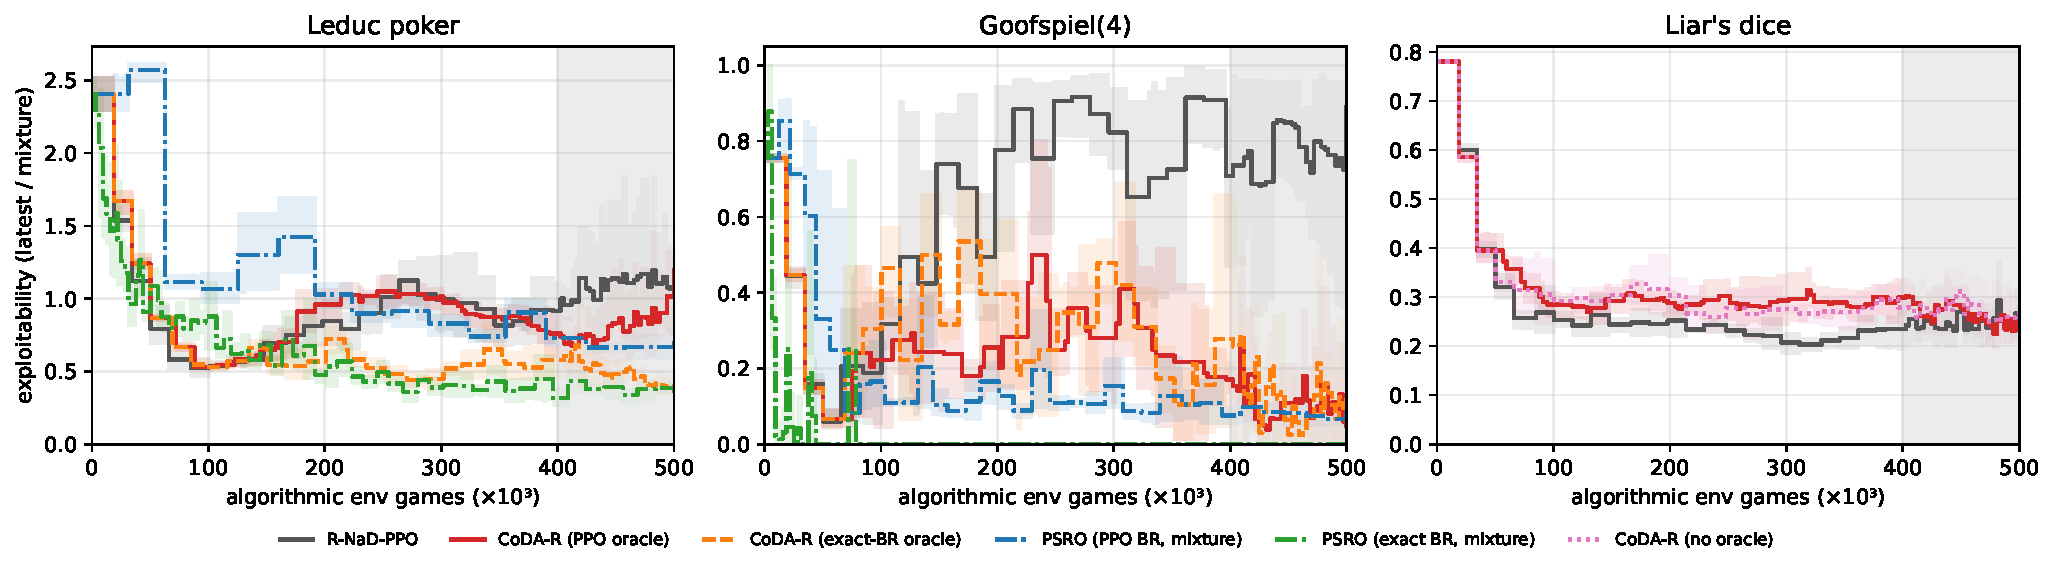
\includegraphics[width=0.9\linewidth]{figures/fig_e1_exploitability.pdf}
\end{center}
\vspace{-6pt}
\caption{Full-tree exploitability at a matched budget (seed mean $\pm$ 95\% CI; gray: last 20\% of the budget). PSRO deploys a multi-network mixture; all other methods deploy the single latest network.}
\label{fig:e1}
\end{figure}

% ----------------------------------------------------------------------
\section{Experiments}
\label{sec:exp}
% ----------------------------------------------------------------------

\subsection{Finite-Dimensional Verification}
\label{sec:exp-theory}

We run the exact algorithm on random skew-symmetric matrix games (up to 64 pure strategies, 1024 steps per cell) and check every inequality of Section~\ref{sec:theory} at every step. Nine groups comprise 3830 cells, 2880 with injected estimation and solver errors. Among about 3.7 million per-step records in the main cells there is not a single violation (Appendix Figure~\ref{fig:theory-cert}); the final $\Expl(\bx_K)$ lies between $10^{-12}$ and $10^{-5}$, and all pool weights go to zero. Breaking any of three mechanisms (a moving dual anchor, a stale mirror snapshot, or frozen pool coefficients) causes thousands of energy-inequality violations, so the checks do detect wrong algorithms. From the counterexample of Proposition~\ref{prop:rps}, the fixed anchor converges within a few steps, while the moving anchor stays at $\Expl=0.5$ and neither the explicit mirror nor $\lambda\equiv0$ converges (Appendix Figure~\ref{fig:theory-mech}).

\subsection{Neural Experiments at a Matched Budget}
\label{sec:exp-neural}
\label{sec:exp-e1}

We implement \codar{} on PPO~\citep{schulman2017ppo}, with each exact object of \S\ref{sec:alg} replaced by a runnable approximation whose error enters $e_k$ or $\delta_k$ (details in Appendix~\ref{app:extra}), and compare it with \rnad{} and PSRO on Leduc poker~\citep{southey2005bayesbluff}, Goofspiel(4)~\citep{ross1971goofspiel}, and Liar's Dice (one die each)~\citep{lisy2015oos} in OpenSpiel~\citep{lanctot2019openspiel}. All PPO methods share the network, the PPO hyperparameters, and $\eta$ (a mechanism comparison, not one of individually tuned methods), and the same budget of $B=5\times10^5$ games, counting all games consumed, oracle games included. We report full-tree exact exploitability (in chips for Leduc) through its mean \texttt{tail\_mean} and maximum \texttt{tail\_worst} over the last 20\% of the budget, as the IQM and bootstrap 95\% CI over 4 seeds~\citep{agarwal2021precipice}. \rnad{} and \codar{} deploy the single latest network, while PSRO deploys a whole-game mixture of networks, which are not directly interchangeable.

\begin{table}[t]
\caption{Matched-budget comparison (IQM [95\% CI], 4 seeds). L: single latest network; M: multi-network mixture. $\Delta$: per-seed paired difference (method $-$ \rnad{}); wins: seeds on which the method is better. Bold: best single-network value per game.}
\label{tab:e1}
\begin{center}
\scriptsize
\setlength{\tabcolsep}{2.3pt}
\begin{tabular}{lcccc}
\toprule
Method & Deploy & tail\_mean & tail\_worst & $\Delta$tail\_mean [CI] (wins) \\
\midrule
\multicolumn{5}{l}{\textit{Leduc}} \\
\rnad{} & L & 0.980 [0.736, 1.684] & 1.224 [1.038, 2.163] & --- \\
\codar{} PPO oracle, $c{=}48$ & L & 0.746 [0.646, 1.206] & 1.217 [0.913, 1.712] & $-0.284$ [$-0.938$, $+0.470$] (3/4) \\
\codar{} exact-BR oracle, $c{=}48$ & L & \textbf{0.492} [0.400, 0.543] & \textbf{0.708} [0.569, 0.845] & $\bm{-0.508}$ [$-1.163$, $-0.273$] (4/4) \\
PSRO, PPO BR & M & 0.656 [0.609, 0.783] & 0.735 [0.647, 0.877] & $-0.359$ [$-0.901$, $-0.057$] (4/4) \\
\midrule
\multicolumn{5}{l}{\textit{Goofspiel(4)}} \\
\rnad{} & L & 0.797 [0.561, 0.953] & 0.901 [0.848, 0.994] & --- \\
\codar{} PPO oracle & L & \textbf{0.083} [0.037, 0.227] & 0.488 [0.320, 0.595] & $-0.659$ [$-0.916$, $-0.446$] (4/4) \\
\codar{} exact-BR oracle & L & 0.115 [0.090, 0.186] & \textbf{0.483} [0.424, 0.638] & $\bm{-0.692}$ [$-0.841$, $-0.375$] (4/4) \\
PSRO, PPO BR & M & 0.072 [0.055, 0.126] & 0.095 [0.061, 0.181] & $-0.705$ [$-0.866$, $-0.506$] (4/4) \\
\midrule
\multicolumn{5}{l}{\textit{Liar's Dice}} \\
\rnad{} & L & 0.259 [0.207, 0.274] & \textbf{0.309} [0.263, 0.406] & --- \\
\codar{} PPO oracle & L & 0.265 [0.231, 0.280] & 0.333 [0.286, 0.350] & $\bm{-0.001}$ [$-0.028$, $+0.073$] (2/4) \\
\codar{} no oracle & L & \textbf{0.256} [0.227, 0.348] & 0.342 [0.276, 0.382] & $+0.023$ [$-0.031$, $+0.074$] (2/4) \\
\bottomrule
\end{tabular}
\end{center}
\end{table}

Table~\ref{tab:e1} and Figure~\ref{fig:e1} give the main results. \textbf{Goofspiel(4).} \rnad{} reaches its lowest point at about $10^5$ games and then degrades to 0.8--0.9; its policy entropy falls below $10^{-4}$ after $2\times10^5$ games (Appendix Figure~\ref{fig:entropy}), so the nearly deterministic policy is fully countered. This is exactly the phase in which the pool of \codar{} gains weight, and the average gain of oracle admissions against latest is 0.13. The tail mean of \codar{} is 0.083, better than \rnad{} on all 4 seeds, although its learner plays about 14\% fewer games. The PSRO (PPO BR) mixture reaches 0.072, on par with \codar{}, indicating that what decides this game is whether the vulnerabilities revealed by the oracle are exploited (exact-BR PSRO uses no games; Appendix Table~\ref{tab:e1full}). The \texttt{tail\_worst} of \codar{} is 0.49, because weight estimates lag behind jumps in the true loss rates (Appendix~\ref{app:diag}). \textbf{Liar's Dice.} The tails of all three methods lie within 0.25--0.27 with fully overlapping CIs, and the median oracle admission gain is 0.002.

\textbf{Leduc and the dual strength.} At $c=6$, the payoff scale leaves the leads of the PPO exploiter too small to earn pool weight (tail 1.235 vs.\ 0.980). With scores normalized over a 26-chip span, 0.8 chips of exploitability is a loss-rate shift of only 0.03, so the closed-form weight $c\mu/2$ is below 0.1. In a pre-specified sweep that changes only $c$ ($c\in\{12,24,48\}$, both oracles; Appendix Table~\ref{tab:csweep}), the IQM of \texttt{tail\_mean} decreases in $c$ under both oracles. At $c=48$, the exact-BR version reaches 0.492, better than \rnad{} on all 4 seeds; the PPO-oracle version reaches 0.746 and is better on 3 seeds, but its CIs overlap and its \texttt{at\_budget} and AUC match \rnad{}; its oracle still finds almost no vulnerabilities, and we cannot tell how much of the extra weight at larger $c$ comes from estimation noise. The $c=48$ results in Table~\ref{tab:e1} use the evaluation seeds and count as a hyperparameter sweep.

\subsection{Controlled Vulnerability Injection and Ablations}
\label{sec:exp-vuln}
\label{sec:exp-abl}

\textbf{Controlled vulnerability injection.} To test whether pool weight exits exactly when the real gain disappears, we inject two pre-trained attackers A and B in turn into a common \rnad{} base on Goofspiel(4), and compare two \codar{} branches (EMA or exact loss rates) against \rnad{} and fixed-mix, which mixes in the attackers at fixed proportions (setup in Appendix~\ref{app:extra}). In both \codar{} branches, $w_A$ and $\ell(\bx;A)-\tfrac12$ drop to 0 in sync, the true lead of A is at most 0.011 once $w_A<0.01$, and the scatter hugs the closed form of Lemma~\ref{lem:dual}(c). Fixed proportions, by contrast, are harmful. After B is injected, fixed-mix overfits the attackers and its tail exploitability rises to 0.45, versus 0.23 for \rnad{} and 0.17 and 0.27 for the \codar{} branches, and these three CIs overlap (the attackers lead by only about 0.05, so repair speed is not compared).

\textbf{Ablations.} In shorter runs, $\eta$ is the most sensitive hyperparameter, and all pool-side ablations differ within the CIs. The moving-anchor \coda{} is worse than \codar{} on Kuhn poker~\citep{kuhn1950poker}, Leduc, and Goofspiel(4) (0.29/0.86/0.96 vs.\ 0.06/0.64/0.04; Appendix~\ref{app:extra}). Because of errors, the certificates are unreliable in the neural setting, where \texttt{latest\_cert} underestimates the truth in 63 of 72 oracle evaluations and does not beat last-checkpoint selection, since the KL proxy does not bound the theoretical term and the exploiter gap $\tau$ is unknown; in PPO they are only diagnostic.

% ----------------------------------------------------------------------
\section{Conclusion}
% ----------------------------------------------------------------------

By placing the moving anchor on the primal side and fixing the dual anchor at pure self-play, \codar{} makes policy movement and pool weight share one budget, which yields single-network last-iterate convergence however opponents enter or leave the pool, with certificates computable during training. It thus combines the openness of population methods with the single-network guarantee of regularized self-play. Black-box opponents can enter or leave the pool at any time, convergence is always carried by the one network being trained, and the method is merely a wrapper around PPO. Empirically, with suitable hyperparameters, \codar{} achieves a significant advantage on Goofspiel(4), where regularized self-play collapses and gets countered, matching a multi-network PSRO mixture with one network, and a considerable advantage on Leduc, while tying on Liar's Dice. Future work includes a Bregman (KL) version of the current Euclidean, normal-form theory, an end-to-end bound on $\delta_k$, a last-iterate rate across pool admissions, and larger games.

\subsubsection*{Reproducibility Statement}
\S\ref{sec:coda}--\ref{sec:theory} give all definitions of the algorithm, and Appendix~\ref{app:proofs} gives all proofs. Anonymized source code is submitted as a zip file in the supplementary material, including the finite-dimensional solver, the PPO implementation, all baselines, the experiment entry points and all hyperparameter configurations, and the scripts that generate all figures and tables.

\subsubsection*{AI Use Statement}
In this work, we used generative AI tools to assist with drafting and polishing the text of the paper, writing and refactoring experiment code, formatting references, and aggregating experiment logs to generate figures and tables. Regarding research content, AI tools were used to refine the formulation of research hypotheses, to assist with derivations and the checking of proof steps, and to assist with interpreting experimental results. The core algorithm, theorem statements, and research design were proposed by the authors. We did not use generative AI to generate synthetic data or to fabricate experimental results. All AI-assisted code was tested and type-checked by the authors, and all AI-assisted proofs, interpretations, and text were manually reviewed item by item by the authors. The authors take responsibility for the entire content of this paper.

\bibliography{references}
\bibliographystyle{iclr2027_conference}

% ----------------------------------------------------------------------
\appendix
\section{Proofs}
\label{app:proofs}
% ----------------------------------------------------------------------

Apart from the minimax theorem and the Hartman--Stampacchia theorem, all proofs use only three tools, namely the polarization identity $\|\bu+\bv\|^2=\|\bu\|^2+\|\bv\|^2+2\bu^\top\bv$, completing the square, and the obtuse-angle principle $\bw=\Proj_C(\bv)\iff(\bv-\bw)^\top(\bu-\bw)\le0\ \forall \bu\in C$. The obtuse-angle principle also yields the monotonicity and nonexpansiveness of the projection. For $\bw=\Proj_C(\bz)$ and $\bw'=\Proj_C(\bz')$, taking $\bu=\bw'$ and $\bu=\bw$ respectively and adding gives
\begin{equation}
(\bz-\bz')^\top(\bw-\bw')\ \ge\ \|\bw-\bw'\|^2\ \ge\ 0 .
\label{eq:monotone}
\end{equation}

\subsection{Proposition~\ref{prop:coda}: \coda{} Converges in the Restricted Game}
\label{app:coda}

Let $L_k(\bx,\brho):=\brho^\top\bell(\bx)-\tfrac1{2c}\|\brho-\brho_k\|^2$. It is affine in $\bx$ and strongly concave in $\brho$, and $X$ and $\simplex_N$ are convex and compact, so by the minimax theorem of \citet{sion1958} a saddle point exists, and since the regularizer does not depend on $\bx$ it can be pulled outside $\min_\bx$:
\[
\min_{\bx}\max_{\brho}L_k(\bx,\brho)=\max_{\brho}\Big[\min_\bx\brho^\top\bell(\bx)-\tfrac1{2c}\|\brho-\brho_k\|^2\Big]=\max_{\brho\in\simplex_N}\Big[\varphi(\brho)-\tfrac1{2c}\|\brho-\brho_k\|^2\Big].
\]
Hence $\brho_{k+1}=\bw_{k+1}$ is a proximal point step on the concave function $\varphi$, and the saddle-point property gives $\bx_{k+1}\in\arg\min_\bx\bw_{k+1}^\top\bell(\bx)$.

\textbf{Monotone ascent.} $\brho_{k+1}$ is an optimal solution of the problem above and $\brho_k$ is feasible, so
\[
\varphi(\brho_{k+1})-\tfrac1{2c}\|\brho_{k+1}-\brho_k\|^2\ \ge\ \varphi(\brho_k)-0 ,
\]
which is the first inequality of the proposition.

\textbf{Finite energy.} Weak duality gives $0\le\varphi(\brho)\le v^*\le1$. Telescoping the first inequality,
\[
\tfrac1{2c}\sum_{k<K}\|\brho_{k+1}-\brho_k\|^2\ \le\ \varphi(\brho_K)-\varphi(\brho_0)\ \le\ 1 ,
\]
so $\sum_k\|\brho_{k+1}-\brho_k\|^2\le2c$; the series converges and its terms tend to zero.

\textbf{In-pool certificate.} Given $\bx_{k+1}$, completing the square gives $\brho_{k+1}=\Proj_{\simplex_N}(\brho_k+c\,\bell(\bx_{k+1}))$. Apply the obtuse-angle principle with $\bu=\be_j$, $j\in\arg\max_i\ell_i(\bx_{k+1})$:
\begin{align*}
&\big(\brho_k+c\,\bell(\bx_{k+1})-\brho_{k+1}\big)^\top(\be_j-\brho_{k+1})\le0\\
\iff{}&
c\,\bell(\bx_{k+1})^\top(\be_j-\brho_{k+1})\ \le\ (\brho_{k+1}-\brho_k)^\top(\be_j-\brho_{k+1}) .
\end{align*}
By Cauchy--Schwarz and the diameter of the simplex, the right-hand side is at most $\sqrt2\,\|\brho_{k+1}-\brho_k\|$; the left-hand side equals $c[\max_i\ell_i(\bx_{k+1})-\brho_{k+1}^\top\bell(\bx_{k+1})]$. The best response gives $\brho_{k+1}^\top\bell(\bx_{k+1})=\min_\bx\brho_{k+1}^\top\bell(\bx)=\varphi(\brho_{k+1})\le v^*$, so
\[
\max_i\ell_i(\bx_{k+1})-v^*\ \le\ \max_i\ell_i(\bx_{k+1})-\varphi(\brho_{k+1})\ \le\ \tfrac{\sqrt2}{c}\|\brho_{k+1}-\brho_k\| .
\]

\textbf{Rate.} For any $\bu\in\simplex_N$ and $t\in(0,1]$, $\bu_t:=\brho_{k+1}+t(\bu-\brho_{k+1})$ is feasible, and the optimality of $\brho_{k+1}$ gives
\[
\varphi(\bu_t)-\tfrac1{2c}\|\bu_t-\brho_k\|^2\ \le\ \varphi(\brho_{k+1})-\tfrac1{2c}\|\brho_{k+1}-\brho_k\|^2 .
\]
Using the concavity of $\varphi$, $\varphi(\bu_t)\ge(1-t)\varphi(\brho_{k+1})+t\varphi(\bu)$, expanding the quadratic term, dividing by $t$, and letting $t\to0^+$, we obtain
\[
\varphi(\bu)-\varphi(\brho_{k+1})\ \le\ \tfrac1c(\brho_{k+1}-\brho_k)^\top(\bu-\brho_{k+1}) .
\]
Taking $\bu=\brho^*\in\arg\max\varphi$ and using the polarization identity $2(\brho_{k+1}-\brho_k)^\top(\brho^*-\brho_{k+1})=\|\brho^*-\brho_k\|^2-\|\brho^*-\brho_{k+1}\|^2-\|\brho_{k+1}-\brho_k\|^2$,
\[
v^*-\varphi(\brho_{k+1})\ \le\ \tfrac1{2c}\big(\|\brho^*-\brho_k\|^2-\|\brho^*-\brho_{k+1}\|^2\big),
\]
and telescoping over $k=0,\dots,K-1$ gives $\sum_{k=1}^K[v^*-\varphi(\brho_k)]\le\|\brho^*-\brho_0\|^2/(2c)\le1/c$. By monotone ascent, $v^*-\varphi(\brho_k)$ is nonincreasing, and the smallest term is at most the average, so $v^*-\varphi(\brho_K)\le1/(cK)$. This bound is independent of $N$, whereas the corresponding bound for Hedge contains a $\log N$ factor.\hfill$\blacksquare$

\subsection{Verification of Proposition~\ref{prop:rps}}
\label{app:rps}

The pool member ties with latest:
\[
\be_1^\top S\by=S_{12}\cdot\tfrac12+S_{13}\cdot\tfrac12=\tfrac12\cdot(-1)\cdot\tfrac12+\tfrac12\cdot1\cdot\tfrac12=0 ,
\]
so $\ell_1(\be_1)=\tfrac12$, the mirror coordinate is also $\tfrac12$, and $c\aug=c(\tfrac12,\tfrac12)$ is a constant vector. Adding a constant vector to a point of the simplex and then projecting returns the point itself (the projection threshold rises uniformly by the same amount), so $\Proj_\simplex(\brho+c\aug)=\brho$ and the dual side stays put. The primal field is
\[
S\big(\lambda \be_1+\tfrac23\by\big)=S\big(\tfrac13,\tfrac13,\tfrac13\big)^\top=0 ,
\]
because the uniform distribution is the Nash strategy of RPS and $S$ maps it to zero; with anchor $\bx_k=\bx$ the proximal term is also zero, so the primal residual is zero. Yet $\Expl(\be_1)=\max_jS_{1j}=\tfrac12$: always playing rock is fully countered by paper.\hfill$\blacksquare$

\subsection{Lemma~\ref{lem:dual}: Properties of the Dual Rule}
\label{app:dual}

Let $\bz:=\be_m+c\aug(\bx)$ and $\bw=\Proj_\simplex(\bz)$.

(a) The obtuse-angle principle says $\be_m=\Proj_\simplex(\bz)$ if and only if $(\bz-\be_m)^\top(\bu-\be_m)\le0$ for all $\bu\in\simplex$. Since $\bz-\be_m=c\aug$, the condition becomes $\aug^\top \bu\le\aug^\top \be_m=\tfrac12$ for all $\bu$; a linear function attains its maximum over the simplex at a vertex, so this means $\max_j\tilde\ell_j\le\tfrac12$. The mirror coordinate is exactly $\tfrac12$, so this is equivalent to $\max_{i\in P}\ell_i\le\tfrac12$.

(b) Move a little weight from member $i$ to the mirror by taking $\bu=\bw+\varepsilon(\be_m-\be_i)$ with $0<\varepsilon\le w_i$, which remains in $\simplex$. The obtuse-angle principle gives
\[
(\bz-\bw)^\top(\bu-\bw)=\varepsilon\big[(z_m-w_m)-(z_i-w_i)\big]\le0
\iff c\,\ell_i-w_i\ \ge\ z_m-w_m=1+\tfrac c2-w_m ,
\]
i.e., $c(\ell_i-\tfrac12)\ge1-w_m+w_i\ge w_i>0$.

(c) The points of $\simplex_2$ are $(s,1-s)$ with $s\in[0,1]$, and their squared distance to $\bz=(\tfrac c2+c\mu,\ 1+\tfrac c2)$,
\[
(\tfrac c2+c\mu-s)^2+(\tfrac c2+s)^2 ,
\]
is a convex quadratic function of $s$ with unconstrained minimizer $s=\tfrac{c\mu}2$; the minimizer over $[0,1]$ is obtained by clipping it to the interval.\hfill$\blacksquare$

With multiple members, the weights are determined by a common projection threshold, and there is no per-member closed form. For example, with $c=4$ and both members at loss rate 0.9, $\bz=(3.6,3.6,3)$ and the candidate is $\bw=(\tfrac12,\tfrac12,0)$; for any $\bu\in\simplex_3$, $(\bz-\bw)^\top(\bu-\bw)=3.1(u_1+u_2-1)+3u_3=-0.1u_3\le0$, so by the obtuse-angle principle it is indeed the projection, and the mirror weight is zero.

\subsection{Unique Solution at Each Step}
\label{app:unique}

\begin{proposition}[Unique solution at each step]
\label{prop:unique}
For any anchor $\bx_k$ and any pool, \eqref{eq:P} has one and only one solution.
\end{proposition}
Uniqueness comes from three facts, namely that the self-play term is skew-symmetric, the pool term is monotone (by the monotonicity of the projection), and the proximal term is $\eta$-strongly monotone; existence follows from the Hartman--Stampacchia theorem. Denote the field $G_k(\bx):=S\bx+A\bw(\bx)_P$.

\textbf{$G_k$ is monotone.}

Self-play term: $(\bx-\bx')^\top S(\bx-\bx')=0$, so $\langle S(\bx-\bx'),\bx-\bx'\rangle=0$.

Pool term: for $\bz=\be_m+c\aug(\bx)$ and $\bz'=\be_m+c\aug(\bx')$, the mirror coordinates coincide and the pool coordinates differ by $c(\ell_i(\bx)-\ell_i(\bx'))=c\,(S\by_i)^\top(\bx-\bx')$, i.e., $(\bz-\bz')_P=c\,A^\top(\bx-\bx')$ and $(\bz-\bz')_m=0$. By \eqref{eq:monotone},
\[
0\le(\bz-\bz')^\top\big(\bw(\bx)-\bw(\bx')\big)=(\bz-\bz')_P^\top\big(\bw(\bx)-\bw(\bx')\big)_P=c\,(\bx-\bx')^\top A\big(\bw(\bx)-\bw(\bx')\big)_P ,
\]
i.e., $\langle A\bw(\bx)_P-A\bw(\bx')_P,\bx-\bx'\rangle\ge0$. After adding $\eta(\bx-\bx_k)$, the whole field satisfies $\langle\cdot,\bx-\bx'\rangle\ge\eta\|\bx-\bx'\|^2$, i.e., it is $\eta$-strongly monotone. This uses the fact that the self-play share does not depend on $\bx$; a share such as $w_m(\bx)$ would turn the self-play term into $w_m(\bx)S\bx$, which is no longer a skew-symmetric quadratic form.

\textbf{Uniqueness.} Suppose $\bx$ and $\bx'$ both solve \eqref{eq:P}. Take the test point $\bx'$ in the inequality for $\bx$, and the test point $\bx$ in the inequality for $\bx'$:
\[
\langle G_k(\bx)+\eta(\bx-\bx_k),\,\bx'-\bx\rangle\ge0,\qquad\langle G_k(\bx')+\eta(\bx'-\bx_k),\,\bx-\bx'\rangle\ge0 .
\]
Adding them gives $\eta\|\bx-\bx'\|^2\le-\langle G_k(\bx)-G_k(\bx'),\bx-\bx'\rangle\le0$, so $\bx=\bx'$.

\textbf{Existence.} $\aug$ is affine and $\bw(\bx)$ is continuous by the nonexpansiveness in \eqref{eq:monotone}, so $G_k$ is continuous; $X$ is compact and convex. A variational inequality with a continuous field on a compact convex set has a solution, which is the Hartman--Stampacchia theorem~\citep{hartman1966,facchinei2003vi}.\hfill$\blacksquare$

\subsection{Lemmas~\ref{lem:A} and~\ref{lem:B}, Theorems~\ref{thm:energy} and~\ref{thm:conv}}
\label{app:lemmas}

\textbf{Proof of Lemma~\ref{lem:A}.} $\bw=\Proj_\simplex(\be_m+c\aug)$. Apply the obtuse-angle principle with $\bu=\be_m\in\simplex$:
\[
\big(\be_m+c\aug-\bw\big)^\top(\be_m-\bw)\le0
\iff\|\be_m-\bw\|^2+c\,\aug^\top(\be_m-\bw)\le0 .
\]
By \eqref{eq:identities}, $\aug^\top \be_m=\tfrac12$ and $\aug^\top \bw=b+\tfrac12$, so $\aug^\top(\be_m-\bw)=-b$. Hence $\|\bw-\be_m\|^2\le c\,b$.\hfill$\blacksquare$

\textbf{Proof of Lemma~\ref{lem:B}.} Take $\bx'=\bx_N$ in \eqref{eq:P} and combine the first two terms into $S\bv$:
\[
\langle S\bv,\,\bx_N-\bx\rangle+\eta\,\dx_k^\top(\bx_N-\bx)\ge0,\qquad
\langle S\bv,\,\bx_N-\bx\rangle=\bx_N^\top S\bv-\bx^\top S\bv=\bx_N^\top S\bv-b .
\]
$\bv=\bx+\sum_iw_i\by_i$ is a nonnegative combination of points in $X$, and by \eqref{eq:nash} each term satisfies $\bx_N^\top S\bz\le0$, so $\bx_N^\top S\bv\le0$. Hence $\eta\,\dx_k^\top(\bx_N-\bx)\ge b-\bx_N^\top S\bv\ge b$.\hfill$\blacksquare$

\textbf{Proof of Theorem~\ref{thm:energy}.} The polarization identity gives
\[
\|\bx_k-\bx_N\|^2=\|\dx_k\|^2+\|\bx_{k+1}-\bx_N\|^2+2\,\dx_k^\top(\bx_N-\bx_{k+1}) ,
\]
and applying Lemma~\ref{lem:B} and then Lemma~\ref{lem:A} to the cross term,
\[
2\,\dx_k^\top(\bx_N-\bx_{k+1})\ \ge\ \tfrac2\eta\,b(\bx_{k+1})\ \ge\ \tfrac{2}{c\eta}\|\bw(\bx_{k+1})-\be_m\|^2 .\eqno\blacksquare
\]

\textbf{Proof of Theorem~\ref{thm:conv}.} Corollary~\ref{cor:sum} gives $a\to0$ and $\|\dx\|\to0$, and substituting into Theorem~\ref{thm:cert}(i) gives $\Expl(\bx_{k+1})\le\tfrac12a+\eta D\|\dx_k\|\to0$. Since $X$ is compact and $\Expl$ is continuous, the limit $\bar \bx$ of any convergent subsequence is Nash; Theorem~\ref{thm:energy} holds with the reference point $\bar \bx$, so $\|\bx_k-\bar \bx\|$ is nonincreasing, and since it tends to zero along the subsequence, it tends to zero along the whole sequence.\hfill$\blacksquare$

\subsection{Theorem~\ref{thm:cert}: Two Certificates}
\label{app:cert}

(i) Take $\by_e\in\arg\max_\by\ell(\bx;\by)$; then $\bx^\top S\by_e=\Expl(\bx)$, and skew-symmetry gives $\by_e^\top S\bx=-\Expl(\bx)$. Take $\bx'=\by_e$ in \eqref{eq:P}, let $\bd:=\by_e-\bx$, and separate the three terms:
\[
\underbrace{(S\bx)^\top \bd}_{\text{self-play}}+\underbrace{(A\bw_P)^\top \bd}_{\text{pool}}+\underbrace{\eta\,\dx^\top \bd}_{\text{proximal}}\ \ge\ 0 .
\]
Self-play term: $(S\bx)^\top \bd=\by_e^\top S\bx-\bx^\top S\bx=-\Expl(\bx)$. Pool term: using $(S\by_i)^\top \bz=\ell_i(\bz)-\tfrac12$,
\[
(A\bw_P)^\top \bd=\sum_iw_i\big(\ell_i(\by_e)-\ell_i(\bx)\big)=\sum_iw_i\big(\ell_i(\by_e)-\tfrac12\big)-b\ \le\ \tfrac12a-b ,
\]
where the last step uses that loss rates are at most 1. Proximal term: by Cauchy--Schwarz and the diameter, $\eta\,\dx^\top \bd\le\eta D\|\dx\|$. Combining the three terms gives $-\Expl(\bx)+\tfrac12a-b+\eta D\|\dx\|\ge0$, and rearranging yields the first inequality; the second inequality uses $b\ge0$.

(ii) Apply the obtuse-angle principle to $\bw=\Proj_\simplex(\be_m+c\aug)$ with $\bu=\be_j$ ($j$ any pool member):
\[
\big(\be_m+c\aug-\bw\big)^\top(\be_j-\bw)\le0\iff c\,\aug^\top(\be_j-\bw)\le(\bw-\be_m)^\top(\be_j-\bw)\le\sqrt2\,\|\bw-\be_m\| .
\]
By \eqref{eq:identities}, the left-hand side equals $c(\ell_j-\tfrac12-b)$, so $\ell_j-\tfrac12\le\frac{\sqrt2}c\|\bw-\be_m\|+b$; moreover, by Lemma~\ref{lem:B} and Cauchy--Schwarz, $b\le\eta\dx^\top(\bx_N-\bx)\le\eta D\|\dx\|$. Taking $j$ to be the largest component, the right-hand side is nonnegative, so taking the positive part does not affect the bound.\hfill$\blacksquare$

\subsection{Theorem~\ref{thm:rate} and Mixed Strategies}
\label{app:rate}

\textbf{Proof of (i).} Let $\alpha_k=\|\bw(\bx_{k+1})-\be_m\|$ and $\beta_k=\|\dx_k\|$. By Theorem~\ref{thm:cert}(i) and $a\le\alpha_k$, $\Expl(\bx_{k+1})\le\tfrac12\alpha_k+\eta D\beta_k$. The minimum is at most the average; applying Cauchy--Schwarz to each of the two sums ($\sum_{k<K}\alpha_k\le\sqrt K\sqrt{\sum\alpha_k^2}$) and substituting Corollary~\ref{cor:sum},
\begin{align*}
\min_{k<K}\Expl(\bx_{k+1})\ &\le\ \frac1K\sum_{k<K}\Big(\tfrac12\alpha_k+\eta D\beta_k\Big)\\
&\le\ \frac{1}{\sqrt K}\Big(\tfrac12\sqrt{\tfrac{c\eta}{2}}+\eta D\Big)\|\bx_0-\bx_N\|\ \le\ \frac{\sqrt{c\eta}/2+2\eta}{\sqrt K},
\end{align*}
where the last step uses $\|\bx_0-\bx_N\|\le\sqrt2$ and $D=\sqrt2$.

\textbf{Monotone residual.} With a fixed pool, two consecutive steps share the same field $G$. Take the test point $\bx_{k+2}$ in \eqref{eq:P} at step $k$ and $\bx_{k+1}$ at step $k+1$:
\[
\langle G(\bx_{k+1})+\eta\dx_k,\ \bx_{k+2}-\bx_{k+1}\rangle\ge0,\qquad\langle G(\bx_{k+2})+\eta\dx_{k+1},\ \bx_{k+1}-\bx_{k+2}\rangle\ge0 .
\]
Adding them, the $G$ part is $\le0$ by monotonicity, leaving $\eta\langle\dx_k-\dx_{k+1},\dx_{k+1}\rangle\ge0$, i.e., $\|\dx_{k+1}\|^2\le\dx_k^\top\dx_{k+1}\le\|\dx_k\|\|\dx_{k+1}\|$, so $\|\dx_{k+1}\|\le\|\dx_k\|$.

\textbf{Proof of (ii).} With the pool unchanged over steps $K-n,\dots,K-1$, the field is the same at all these steps, so $\|\dx_k\|$ is nonincreasing there by the monotone residual. Summing the energy inequality \eqref{eq:energy} from $\bx_{K-n}$ gives $n\|\dx_{K-1}\|^2\le\sum_{k=K-n}^{K-1}\|\dx_k\|^2\le\|\bx_{K-n}-\bx_N\|^2\le2$, i.e., $\beta:=\|\dx_{K-1}\|\le\sqrt{2/n}$. At $\bx=\bx_K$, Lemma~\ref{lem:B} and Cauchy--Schwarz give $b(\bx)\le\eta D\beta$, and Lemma~\ref{lem:A} with $a^2\le\|\bw-\be_m\|^2$ gives $a(\bx)\le\sqrt{c\,b(\bx)}\le\sqrt{c\eta D\beta}$. Substituting into Theorem~\ref{thm:cert}(i),
\[
\Expl(\bx_K)\ \le\ \tfrac12\sqrt{c\eta D\beta}+\eta D\beta\ \le\ \sqrt{c\eta/2}\;n^{-1/4}+2\eta\,n^{-1/2},
\]
using $D=\sqrt2$. The residual itself decays at rate $n^{-1/2}$, but the pool weight only at rate $n^{-1/4}$, which dominates.\hfill$\blacksquare$

Besides latest $\bx_{k+1}$ (a single network), each step yields two deployable mixtures, the current mixture $\bq_{k+1}:=\bv_{k+1}/t_k$ and the time average
\[
\bar{\bq}_K:=\frac1{T_K}\sum_{k<K}\bv_{k+1},\qquad T_K:=\sum_{k<K}t_k .
\]
In sequential games, a mixture becomes a behavior strategy via reach probabilities~\citep{kuhn1953}. Both mixtures also converge.
\begin{proposition}[Mixed strategies]
\label{prop:mix}
(i) The per-step mixture satisfies $t_k\Expl(\bq_{k+1})\le\eta D\|\dx_k\|$. Since $t_k\ge1$, $\Expl(\bq_{k+1})\le\eta D\|\dx_k\|\to0$, and this conclusion does not require $a\to0$.\\
(ii) The time average satisfies
\[
\Expl(\bar{\bq}_K)\ \le\ \frac{\eta\max_\by\|\bx_0-\by\|^2}{2T_K}\ \le\ \frac{\eta}{T_K},
\]
and $T_K=K+\sum_{k<K}a(\bx_{k+1})\ge K$.\\
(iii) With the errors of \S\ref{sec:inexact}, these bounds become
\[
t_k\Expl(\bq_{k+1})\ \le\ \eta D\|\dx_k\|+\delta_k+ae_k,\qquad
\Expl(\bar{\bq}_K)\ \le\ \Big[\eta+\textstyle\sum_{k<K}(\delta_k+a_{k+1}e_k)\Big]\big/T_K .
\]
\end{proposition}
Unlike Theorem~\ref{thm:cert}(i), (i) has no $\tfrac12a$ term, because that term comes from the crude bound that the loss rate of the exploiter against a pool member is at most 1, which is not needed once the deployed object is the mixture formed from the coefficients of the algorithm. (ii) is the standard order for averaged iterates of the proximal point method~\citep{rockafellar1976ppa,nemirovski2004prox}, except that under the augmented structure the pool cross terms cancel exactly and pool admissions do not break the telescoping sum. (iii) is proved in Appendix~\ref{app:inexact}.

\textbf{Proof of (i).} $\bq_{k+1}=\bv_{k+1}/t_k\in X$, because $\bv$ is a nonnegative combination of points in $X$ with total mass $t_k\ge1$. For any $\by\in X$, take $\bx'=\by$ in \eqref{eq:P}:
\[
\by^\top S\bv-\underbrace{\bx^\top S\bv}_{=b}+\eta\,\dx^\top(\by-\bx)\ge0
\ \Longrightarrow\
-\by^\top S\bv\ \le\ -b+\eta\,\dx^\top(\by-\bx)\ \le\ \eta D\|\dx\| .
\]
By skew-symmetry, the left-hand side equals $\bv^\top S\by=t\,\bq^\top S\by$, and maximizing over $\by$ gives $t_k\Expl(\bq_{k+1})\le\eta D\|\dx_k\|$.

\textbf{Proof of (ii).} The intermediate step above, $-\by^\top S\bv_{k+1}\le\eta\dx_k^\top(\by-\bx_{k+1})$, holds at every step. Using the polarization identity (with reference point $\by$),
\[
2\,\dx_k^\top(\by-\bx_{k+1})=\|\bx_k-\by\|^2-\|\bx_{k+1}-\by\|^2-\|\dx_k\|^2\ \le\ \|\bx_k-\by\|^2-\|\bx_{k+1}-\by\|^2 ,
\]
and telescoping over $k<K$,
\[
T_K\,\bar{\bq}_K^\top S\by=-\by^\top S\sum_{k<K}\bv_{k+1}\ \le\ \tfrac\eta2\big(\|\bx_0-\by\|^2-\|\bx_K-\by\|^2\big)\ \le\ \tfrac\eta2\|\bx_0-\by\|^2\ \le\ \eta .
\]
Divide both sides by $T_K$ and maximize over $\by$; $T_K\ge K$ because every $t_k=1+a(\bx_{k+1})\ge1$.\hfill$\blacksquare$

\subsection{Theorem~\ref{thm:inexact} and the Two Convergence Results}
\label{app:inexact}

Let $\hat b:=\sum_iw_{k+1,i}(\hat\ell_{k,i}-\tfrac12)$ denote the pool pressure computed from the estimated loss rates, while $a$ and $b$ are defined with the actual weights and the true loss rates.

\textbf{Energy inequality.} Lemma~\ref{lem:A} holds as usual for the vector that is actually projected (the proof is the same, with $\aug$ replaced by $\hat{\bell}$), giving $\|\bw_{k+1}-\be_m\|^2\le c\hat b$. Switching back to the true values,
\[
\hat b-b=\sum_iw_{k+1,i}\big(\hat\ell_{k,i}-\ell_i(\hat \bx_{k+1})\big)\le\sum_iw_{k+1,i}\,e_k=a\,e_k ,
\]
since only the pool coordinates carry error (the mirror coordinate is always $\tfrac12$), which makes this tighter than the generic $2e$ bound. Lemma~\ref{lem:B} with $-\delta_k$: taking $\bx'=\bx_N$ in the relaxed \eqref{eq:P}, we again have $\bx_N^\top S\hat \bv\le0$, which gives $\eta\dx^\top(\bx_N-\hat \bx)\ge b-\delta_k$. Chaining these,
\[
\eta\,\dx^\top(\bx_N-\hat \bx)\ \ge\ b-\delta_k\ \ge\ \hat b-ae_k-\delta_k\ \ge\ \tfrac1c\|\bw_{k+1}-\be_m\|^2-ae_k-\delta_k ,
\]
and substituting into the polarization identity gives the energy inequality.

\textbf{Certificates.} Repeat the proofs of Theorem~\ref{thm:cert} and Proposition~\ref{prop:mix}(i)(ii) with two substitutions; this also proves Proposition~\ref{prop:mix}(iii). The right-hand side of \eqref{eq:P} changes from $0$ to $-\delta_k$, which adds $\delta_k$ to every certificate. Wherever $-b\le0$ was used, we now only have $\hat b\ge0$, so we use $-b\le-\hat b+ae_k\le ae_k$, which adds $ae_k$ to the latest certificate and to each of the two mixture certificates. In-pool certificate: the obtuse-angle principle applied to $\be_m+c\hat{\bell}$ gives $\hat\ell_j-\tfrac12\le\frac{\sqrt2}c\|\bw-\be_m\|+\hat b$; switching back to the true values uses $\ell_j\le\hat\ell_j+e_k$ and $\hat b\le b+ae_k\le b+e_k$, for a total of $2e_k$, and finally $b\le\eta D\|\dx\|+\delta_k$.

\textbf{Summable errors $\Rightarrow$ convergence.} If $\sum_k(\delta_k+a_{k+1}e_k)<\infty$, summing the energy inequality gives $\sum\|\dx_k\|^2<\infty$ and $\sum\|\bw_{k+1}-\be_m\|^2<\infty$, so $a\to0$ and $\dx\to0$, and substituting into the latest certificate gives $\Expl(\hat \bx_{k+1})\to0$. For convergence of the whole sequence, define
\[
E_k:=\|\bx_k-\bx_N\|^2+\tfrac2\eta\sum_{j\ge k}\big(\delta_j+a_{j+1}e_j\big);
\]
the energy inequality gives $E_{k+1}\le E_k$, and since the tail sum tends to zero, $E_k$ and $\|\bx_k-\bx_N\|^2$ have the same limit; then take the limit along a subsequence converging to a Nash strategy. Summable errors do not restore the monotonicity of the residuals.

\textbf{Constant errors $\Rightarrow$ neighborhood.} If $\delta_k\le\delta$ and $e_k\le e$, summing the energy inequality and dividing by $K$ gives
\[
\min_{k<K}\Big[\|\dx_k\|^2+\tfrac{2}{c\eta}\|\bw_{k+1}-\be_m\|^2\Big]\le\tfrac2K+\tfrac2\eta(\delta+e) .
\]
This is a statement about $\min_{k<K}$. Re-summing over an arbitrary suffix yields a $\liminf$-type statement, but it does not imply that the iterates stay in the neighborhood from some point onward.\hfill$\blacksquare$

\subsection{The Role of the Oracle}
\label{app:oracle}

Theorem~\ref{thm:conv} shows that exploiters can enter or leave the pool freely without breaking convergence. On top of this, the oracle does two things. It provides directed pressure (with a single member, the admission weight is $\operatorname{clip}(c\mu/2,0,1)$), and it provides measurable evidence, namely the admission gain $g:=[\ell(\hat \bx;\hat \by)-\max_{i\in P}\ell_i(\hat \bx)]^+$. If the oracle falls short of the worst-case opponent by only $\tau$, i.e., $\max_\by\ell(\hat \bx;\by)\le\ell(\hat \bx;\hat \by)+\tau$, then a one-line decomposition gives
\[
\Expl(\hat \bx)\le\Big[\max_{i\in P}\ell_i(\hat \bx)-\tfrac12\Big]^++g+\tau ;
\]
$\tau$ is not measurable for a neural exploiter, and this is the source of the bridge proxy underestimating the true value in \S\ref{sec:exp-abl}.

% ----------------------------------------------------------------------
\section{Comparison with Mainstream Methods}
\label{app:related}
% ----------------------------------------------------------------------

\begin{table}[!htbp]
\caption{Comparison with mainstream methods.}
\label{tab:related}
\begin{center}
\footnotesize
\resizebox{\linewidth}{!}{%
\begin{tabular}{lllcccc}
\toprule
 & Deployed object & Equilibrium carrier & Modifies RL core & Nontransitive memory & Actively finds holes & Online certificate \\
\midrule
PSRO / DO & Mixture & External meta-solver & No & Yes & Yes & Within meta-game \\
Hedge/MWU pool weights$^{\dagger}$ & Mixture or time average & Accumulated weights (moving dual anchor) & No & Yes & Yes & Time-average regret \\
PFSP / League & Single network & None & No & Yes & Yes & None \\
NFSP & Average network & Average network & Yes & Implicit & No & None \\
R-NaD / MMD & Single network & Moving anchor & Yes & No & No & Primal residual \\
\coda{} (moving dual anchor) & Single network & Moving anchor on sampling simplex & No & Yes & Yes & In-pool \\
\textbf{\codar{}} & Single network or mixture & Primal moving anchor + fixed dual anchor $\be_m$ & Wrapper & Yes & Yes & In-pool and full-game \\
\bottomrule
\end{tabular}}
\par\smallskip
\parbox{\linewidth}{\scriptsize $^{\dagger}$Including the Hedge/PRD meta-solvers of PSRO~\citep{lanctot2017psro}, the opponent sampler of OpenAI Five~\citep{openai2019dota}, APSRO~\citep{mcaleer2022anytime}, and ODO~\citep{dinh2022odo}.}
\end{center}
\end{table}

% ----------------------------------------------------------------------
\section{Additional Experimental Results}
\label{app:extra}
% ----------------------------------------------------------------------

\textbf{Implementation and evaluation protocol.} The PPO implementation~\citep{schulman2017ppo} (with GAE~\citep{schulman2016gae} for advantage estimation) follows the procedure of \S\ref{sec:alg}, replacing each exact object with a runnable approximation whose error is absorbed into $e_k$ or $\delta_k$. One outer step contains 32 rollouts. After each rollout, the game outcomes are used to update the loss-rate estimates $\hat{\bell}$ and to re-project, and the next rollout samples opponents accordingly and applies importance weighting. The opponent of the mirror arm is a frozen copy of the current parameters, the proximal term takes the form of R-NaD-style reward shaping, and the policy anchor is updated at the end of each outer step. The oracle trains exploiters with PPO, and the upper-bound control uses full-tree exact best responses instead. In the implementation, $a$ and $\|\bw-\be_m\|$ can be read off directly, but the primal residual has only a KL proxy and $\delta_k$ has no end-to-end bound, as is also the case for neural \rnad{} and PSRO. The budget of $B=5\times10^5$ games counts the games the algorithm actually consumes, including learner games, exploiter training, admission evaluation, and the meta-matrix games of PSRO; \codar{} spends about 14\% of its budget on the oracle, and its learner plays correspondingly fewer games. Exploitability is measured in chips for Leduc; the payoffs of the other games are $\pm1$.

\textbf{Short and long runs.} The long-run comparison of \S\ref{sec:exp-e1}, the dual-strength sweep on Leduc, and the vulnerability injection of \S\ref{sec:exp-vuln} use the same setup; the ablations, the comparison with \coda{}, and the neural certificate proxies come from earlier short runs (96 or 192 rollouts). The main difference between the two lies in the dual-side loss-rate estimator. Short runs use an EMA with a fixed step size ($\beta=0.1$) and a pool capacity of 16; long runs instead use an EMA whose step size adapts to the number of games, reset the history when the estimate changes abruptly, reserve a small fraction of games to probe zero-weight members, and use a pool capacity of 8. In addition, the horizontal axis of short runs counts pool-evaluation games that are used only for logging.

\textbf{Controlled vulnerability injection.} Results are shown in Figure~\ref{fig:e2}, Figure~\ref{fig:weight-hole}, and Table~\ref{tab:e2}. For each seed, we first train \rnad{} for 64 rollouts to obtain a common base, and train attacker A with PPO so that the loss rate of the base rises to 0.55--0.57; four branches then start from the same base with newly created optimizers and each train for 96 rollouts, with A injected at rollout 0 and B (an attacker trained against the policy of the reference branch at rollout 48) injected at rollout 48. The proportions of fixed-mix (fixmix in the table) are fixed before the experiment, namely $(w_m,w_A)=(0.65,0.35)$ after A is injected and $(w_m,w_A,w_B)=(0.50,0.25,0.25)$ after B is injected. The value 0.35 is the closed-form initial weight computed from an expected lead of 0.12 and $c=6$; the actual attackers lead by only 0.05--0.07, so fixed-mix gives A about twice the initial weight of \codar{} (0.12--0.20). coda\_r\_exact overwrites the estimates with the exact $\ell_i$ at every rollout ($e_k=0$). B finds no vulnerability on 3 of 4 seeds, and the $T_{\rm fix}$ of all branches is close to immediate repair. The exact-loss-rate version is not better than the EMA version, and the difference is within the CIs.

\textbf{Ablations, comparison with \coda{}, and certificate proxies.} The ablations are shown in Figure~\ref{fig:ablations} (96 rollouts), the comparison with the moving-anchor \coda{} in Figure~\ref{fig:v1}, and the neural certificate proxies in Figure~\ref{fig:bridge}. \codar{} and \rnad{} show similar trends as $\eta$ varies. Of the two forms of the proximal term, loss KL is better on Leduc and reward shaping is significantly better on Goofspiel(4); the main experiments use reward shaping for both methods. Freezing the mirror for a whole period is worse on Leduc (1.36 vs.\ 1.14); the differences for freezing the pool coefficients and for switching the oracle on or off are all within the CIs. Among the negative results, the bridge proxy $[\max_P\ell_i-\tfrac12]^++g$ falls below the true value in 55 of 72 oracle evaluations; selecting the checkpoint at the minimum of \texttt{latest\_cert} is worse on Leduc than taking the last one ($+0.145$ [0.101, 0.678], Figure~\ref{fig:ckpt}).

\subsection{Estimator and Oracle Diagnostics}
\label{app:diag}

Table~\ref{tab:diag} explains two phenomena in the main results. On Goofspiel(4), the oracle does find vulnerabilities (mean $g$ of 0.13), but in 54 of the 61 cases where the true loss rate against a member jumped above 0.52, the weight of that member was below 0.01 at the time; the lag of the estimator is the source of the occasional spikes in \texttt{tail\_worst}, and it is also the measured form of $e_k$ in Theorem~\ref{thm:inexact}. On Leduc, $g$ is always 0 for the PPO oracle, so the pool barely takes part in training; the true loss rates against exact-BR members do exceed 0.52 (96 times), but the closed-form weight is too small at $c=6$, and after scaling up to $c=48$ the holes drop to 5 and the pool mass rises to 0.29.

\begin{table}[!htbp]
\caption{Pool diagnostics of each \codar{} cell in the long-run comparison. $g$ is the gain against latest at oracle admission; holes is the number of member occurrences with true loss rate $>0.52$ at evaluation ticks, with the number of those whose weight was $<0.01$ at the time in parentheses; dual regret $=\max_j\ell_j-\sum_jw_j\ell_j$ ($\bw$ normalized within the pool).}
\label{tab:diag}
\begin{center}
\footnotesize
\resizebox{\linewidth}{!}{%
\begin{tabular}{llcccccc}
\toprule
Environment & Method & \#oracle & mean $g$ & $g>0.02$ & pool\_mass & holes (missed) & dual regret mean / p90 \\
\midrule
Goofspiel(4) & PPO oracle & 24 & 0.127 & 21 & 0.040 & 61 (54) & 0.044 / 0.146 \\
Goofspiel(4) & exact-BR oracle & 28 & 0.116 & 18 & 0.039 & 64 (50) & 0.035 / 0.120 \\
Leduc & PPO oracle, $c{=}6$ & 24 & 0.000 & 0 & 0.023 & 0 & 0.004 / 0.011 \\
Leduc & exact-BR oracle, $c{=}6$ & 28 & 0.019 & 14 & 0.065 & 96 (30) & 0.008 / 0.020 \\
Leduc & exact-BR oracle, $c{=}48$ & 28 & 0.010 & 2 & 0.291 & 5 (2) & 0.006 / 0.014 \\
Liar's Dice & PPO oracle & 28 & 0.018 & 7 & 0.066 & n/a & n/a \\
\bottomrule
\end{tabular}}
\end{center}
\end{table}

\subsection{Figures and Tables}

\begin{figure}[!htbp]
\begin{center}
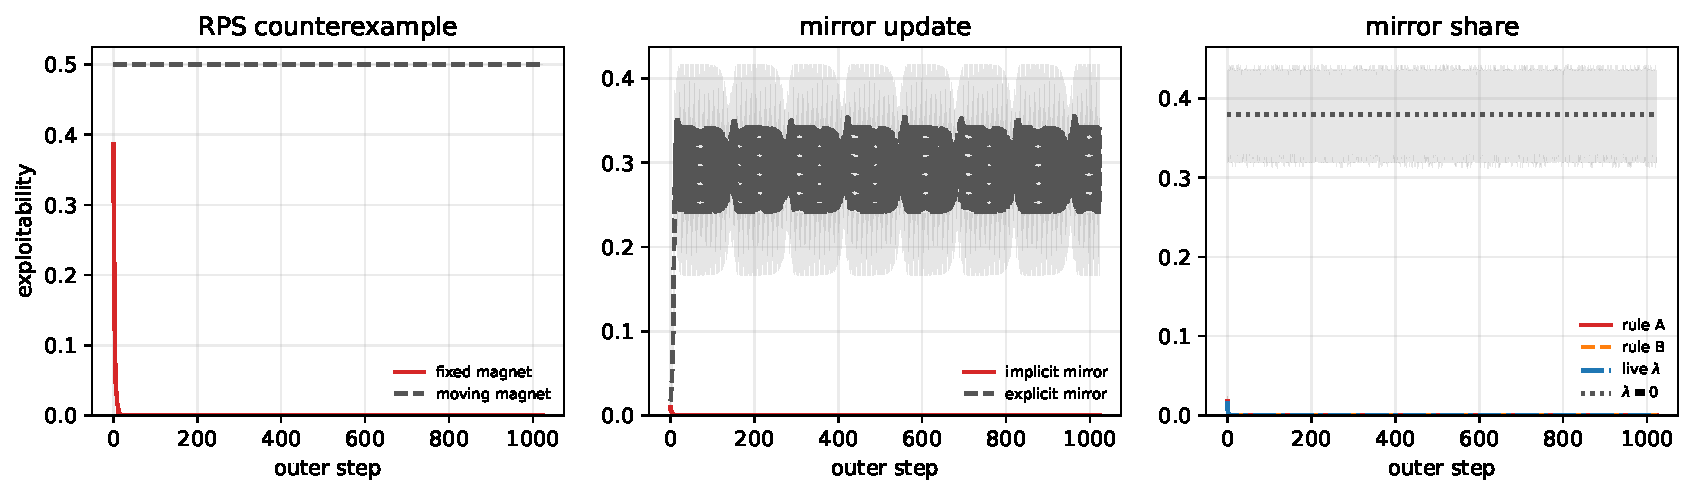
\includegraphics[width=0.76\linewidth]{figures/fig_theory_mechanisms.pdf}
\end{center}
\caption{Finite-dimensional mechanism comparison (seed mean $\pm$ CI; vertical axis $\Expl(\bx_k)$). Left: fixed versus moving anchor, starting from the RPS counterexample point. Middle: implicit versus explicit mirror. Right: share Rules A and B, real-time $\lambda$, and $\lambda\equiv0$.}
\label{fig:theory-mech}
\end{figure}

\begin{figure}[!htbp]
\begin{center}
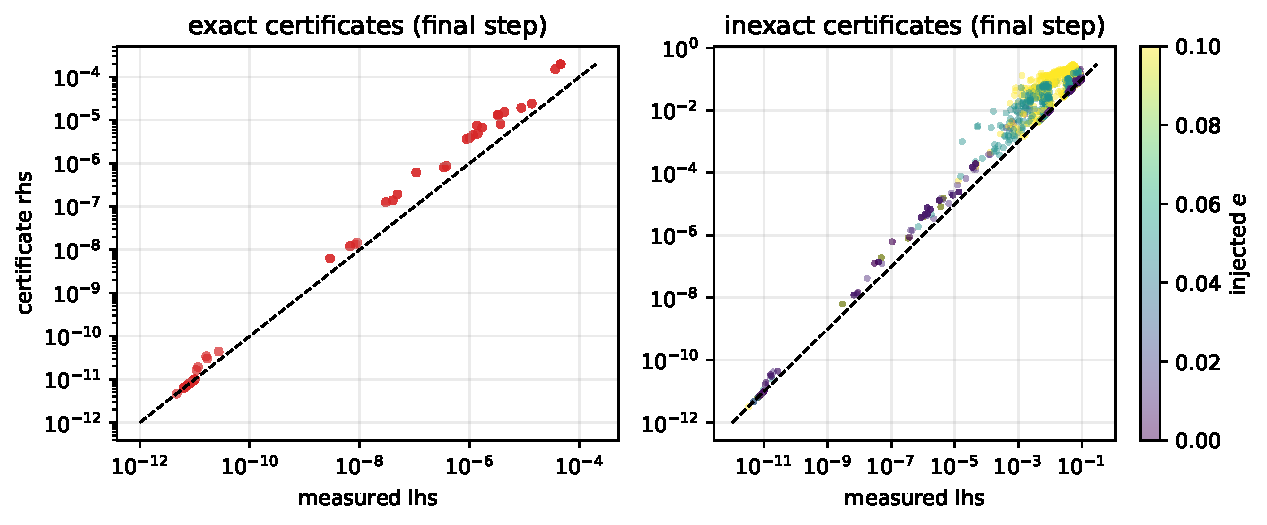
\includegraphics[width=0.6\linewidth]{figures/fig_theory_certificates.pdf}
\end{center}
\caption{Certificates at the last step of the finite-dimensional experiments. The horizontal axis is the measured left-hand side, the vertical axis is the right-hand side of the certificate, and the dashed line is the diagonal $y=x$. Left: exact cells. Right: cells with errors, colored by the injected $e$.}
\label{fig:theory-cert}
\end{figure}

\begin{figure}[!htbp]
\begin{center}
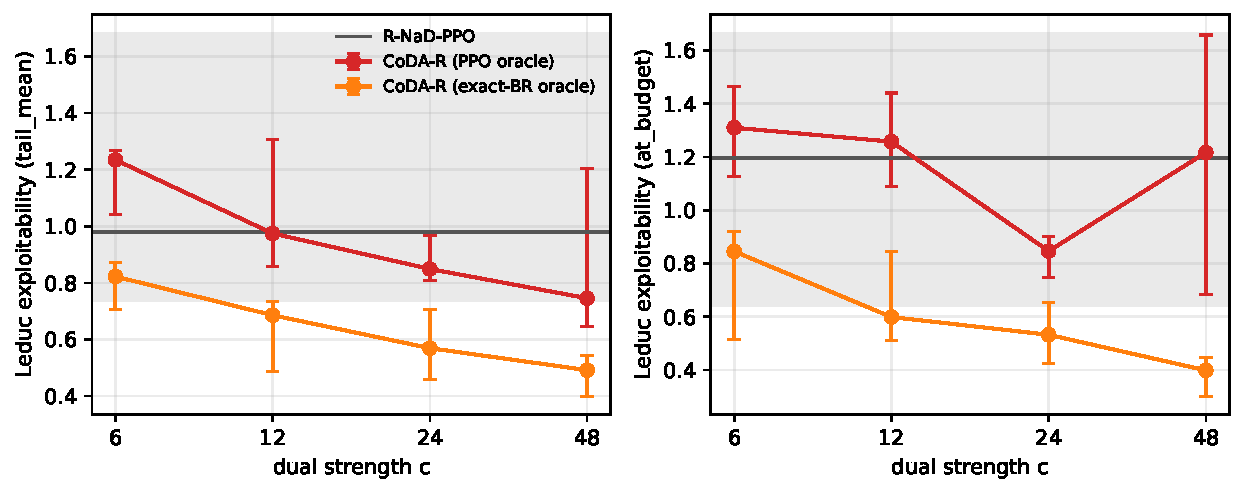
\includegraphics[width=0.6\linewidth]{figures/fig_e3_c_sweep.pdf}
\end{center}
\caption{Dual-strength sweep on Leduc (IQM $\pm$ 95\% CI). The gray line and shading are \rnad{}. Left: \texttt{tail\_mean}. Right: \texttt{at\_budget}.}
\label{fig:csweep}
\end{figure}

\begin{figure}[!htbp]
\begin{center}
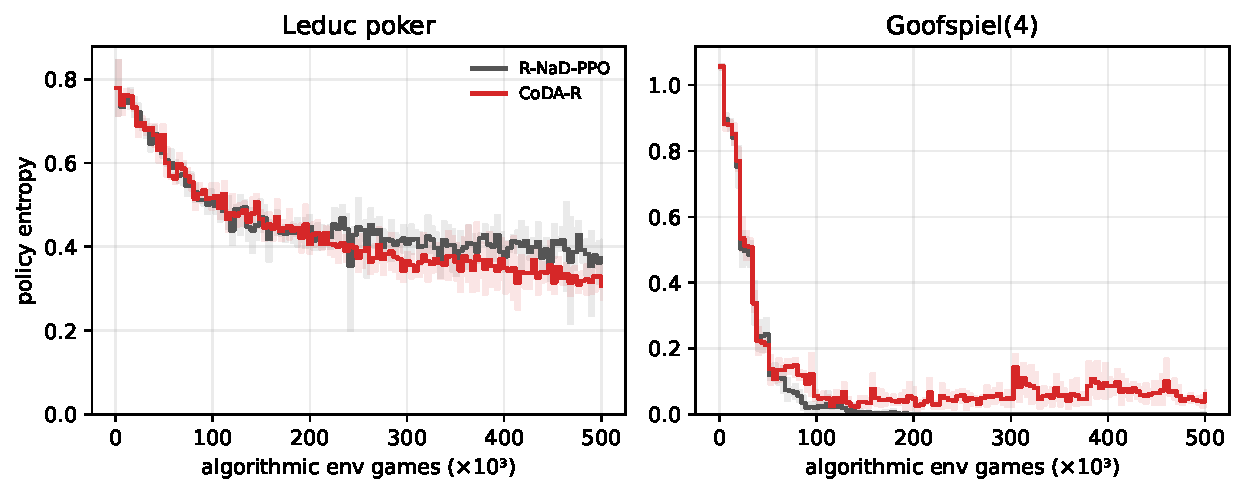
\includegraphics[width=0.62\linewidth]{figures/fig_entropy.pdf}
\end{center}
\caption{Policy entropy in the matched-budget long-run comparison (seed mean $\pm$ CI). On Goofspiel(4), the entropy of \rnad{} falls below $10^{-4}$ after $2\times10^5$ games, in step with the degradation of its exploitability; \codar{} stays at 0.05--0.1.}
\label{fig:entropy}
\end{figure}

\begin{table}[!htbp]
\caption{Full metrics of the matched-budget long-run comparison ($B=5\times10^5$, IQM [95\% CI], $n=4$). AUC is the integral over $[0,B]$ with previous-value hold, divided by $B$. Bold marks the best value among single-network methods in each game.}
\label{tab:e1full}
\begin{center}
\scriptsize
\setlength{\tabcolsep}{4pt}
\begin{tabular}{lcccc}
\toprule
Method & Deploy & at\_budget & tail\_mean & AUC \\
\midrule
\multicolumn{5}{l}{\textit{Leduc}} \\
\rnad{} & L & 1.196 [0.637, 1.666] & 0.980 [0.736, 1.684] & 0.937 [0.860, 1.081] \\
\codar{} PPO oracle, $c{=}48$ & L & 1.217 [0.684, 1.658] & 0.746 [0.646, 1.206] & 0.930 [0.852, 0.986] \\
\codar{} exact-BR oracle, $c{=}48$ & L & \textbf{0.398} [0.301, 0.445] & \textbf{0.492} [0.400, 0.543] & \textbf{0.681} [0.637, 0.706] \\
PSRO, PPO BR & M & 0.650 [0.637, 0.877] & 0.656 [0.609, 0.783] & 1.123 [1.114, 1.148] \\
PSRO, exact BR & M & 0.353 [0.304, 0.419] & 0.374 [0.369, 0.394] & 0.616 [0.558, 0.634] \\
\midrule
\multicolumn{5}{l}{\textit{Goofspiel(4)}} \\
\rnad{} & L & 0.869 [0.827, 0.990] & 0.797 [0.561, 0.953] & 0.653 [0.579, 0.707] \\
\codar{} PPO oracle & L & \textbf{0.014} [0.000, 0.165] & \textbf{0.083} [0.037, 0.227] & \textbf{0.244} [0.211, 0.283] \\
\codar{} exact-BR oracle & L & 0.079 [0.000, 0.323] & 0.115 [0.090, 0.186] & 0.290 [0.239, 0.330] \\
PSRO, PPO BR & M & 0.088 [0.054, 0.115] & 0.072 [0.055, 0.126] & 0.173 [0.156, 0.191] \\
PSRO, exact BR & M & $<10^{-15}$ & $<10^{-15}$ & 0.018 [0.011, 0.023] \\
\midrule
\multicolumn{5}{l}{\textit{Liar's Dice}} \\
\rnad{} & L & 0.272 [0.216, 0.291] & 0.259 [0.207, 0.274] & \textbf{0.279} [0.268, 0.282] \\
\codar{} PPO oracle & L & \textbf{0.251} [0.179, 0.257] & 0.265 [0.231, 0.280] & 0.317 [0.295, 0.345] \\
\codar{} no oracle & L & 0.253 [0.230, 0.353] & \textbf{0.256} [0.227, 0.348] & 0.310 [0.304, 0.337] \\
\bottomrule
\end{tabular}
\end{center}
\end{table}

\begin{table}[!htbp]
\caption{Dual-strength sweep on Leduc ($B=5\times10^5$, IQM [95\% CI], $n=4$; $c=6$ is taken from the main-experiment runs). pool\_mass is the mean of $a$ over the whole run, and est err is the mean of $|\hat\ell_i-\ell_i|$ at evaluation ticks. Bold marks the best \texttt{at\_budget} and \texttt{tail\_mean} under each oracle.}
\label{tab:csweep}
\begin{center}
\footnotesize
\begin{tabular}{llcccc}
\toprule
oracle & $c$ & at\_budget & tail\_mean & pool\_mass & est err \\
\midrule
PPO & 6 & 1.310 [1.127, 1.464] & 1.235 [1.041, 1.269] & 0.023 & 0.010 \\
PPO & 12 & 1.257 [1.089, 1.440] & 0.975 [0.860, 1.305] & 0.039 & 0.010 \\
PPO & 24 & \textbf{0.846} [0.746, 0.902] & 0.849 [0.808, 0.967] & 0.070 & 0.010 \\
PPO & 48 & 1.217 [0.684, 1.658] & \textbf{0.746} [0.646, 1.206] & 0.123 & 0.010 \\
\midrule
exact BR & 6 & 0.845 [0.513, 0.921] & 0.823 [0.707, 0.873] & 0.065 & 0.011 \\
exact BR & 12 & 0.599 [0.509, 0.843] & 0.686 [0.486, 0.735] & 0.107 & 0.010 \\
exact BR & 24 & 0.532 [0.426, 0.652] & 0.570 [0.460, 0.708] & 0.175 & 0.009 \\
exact BR & 48 & \textbf{0.398} [0.301, 0.445] & \textbf{0.492} [0.400, 0.543] & 0.291 & 0.010 \\
\bottomrule
\end{tabular}
\end{center}
\end{table}

\begin{table}[!htbp]
\caption{Controlled vulnerability injection (Goofspiel(4), $n=4$, IQM [95\% CI]). $T_{\rm fix}$ is the rollout index at which $\ell\le0.52$ first holds for three consecutive rollouts; recur$_A$ is the maximum of $\ell(\bx;A)-\tfrac12$ over $r\ge56$; gap is the maximum true gain of A while $w_A<0.01$; est err is the mean of $|\hat\ell_A-\ell(\bx;A)|$. Lower is better for the first four columns, and bold marks the best value in each column; gap and est err are diagnostics of \codar{} and are not compared.}
\label{tab:e2}
\begin{center}
\footnotesize
\setlength{\tabcolsep}{3.5pt}
\begin{tabular}{lcccccc}
\toprule
Branch & $T_{\rm fix,A}$ & recur$_A$ & expl\_tail & expl\_worst\_tail & gap & est err \\
\midrule
rnad & 3.5 & 0.0073 & 0.232 [0.186, 0.326] & 0.387 [0.221, 0.569] & --- & --- \\
fixmix & \textbf{2.0} & 0.0138 & 0.450 [0.201, 0.574] & 0.521 [0.289, 0.614] & --- & --- \\
coda\_r\_ema & 6.0 & 0.0080 & \textbf{0.167} [0.072, 0.272] & \textbf{0.272} [0.099, 0.514] & 0.0115 & 0.0062 \\
coda\_r\_exact & 3.5 & \textbf{0.0056} & 0.267 [0.185, 0.339] & 0.404 [0.393, 0.450] & 0.0048 & 0 \\
\bottomrule
\end{tabular}
\end{center}
\end{table}

\begin{figure}[!htbp]
\centering
\begin{minipage}[b]{0.6\linewidth}
\centering
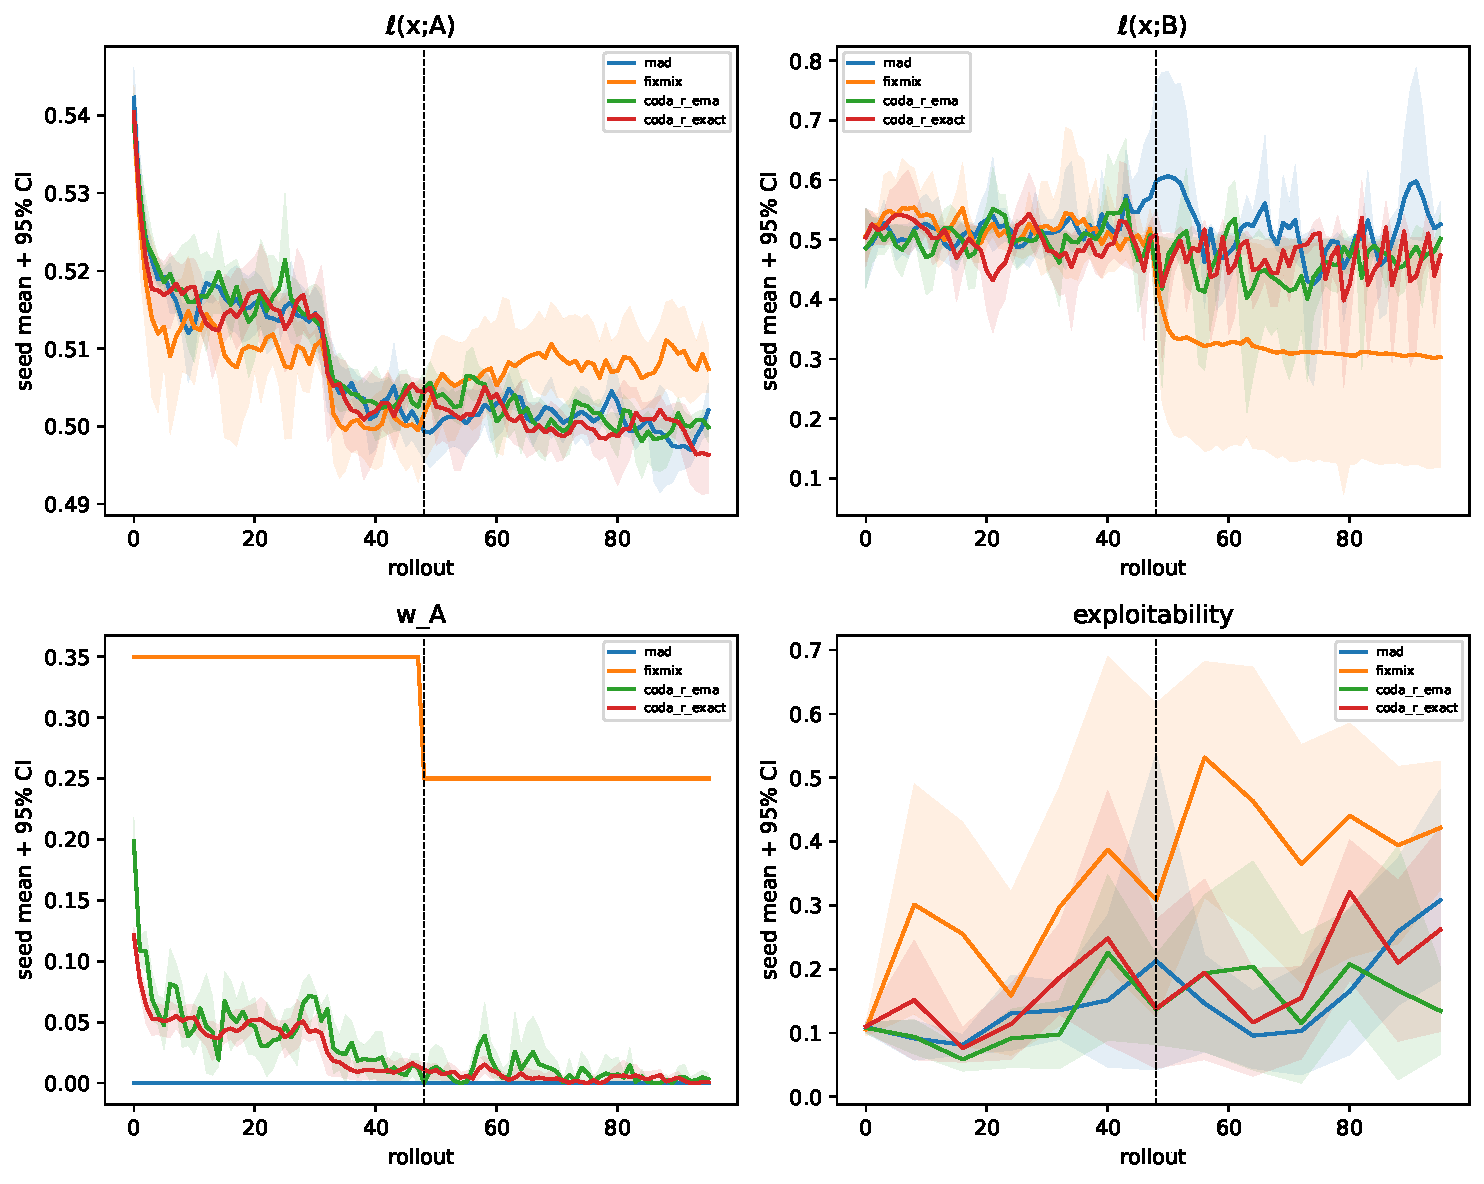
\includegraphics[width=\linewidth]{figures/fig_e2_vuln_panels.pdf}
\caption{Controlled vulnerability injection (Goofspiel(4), seed mean $\pm$ 95\% CI; the dashed line marks rollout 48, where B is injected). Top left: $\ell(\bx;A)$. Top right: $\ell(\bx;B)$. Bottom left: $w_A$ (fixed proportion for fixmix). Bottom right: full-tree exploitability.}
\label{fig:e2}
\end{minipage}\hfill
\begin{minipage}[b]{0.37\linewidth}
\centering
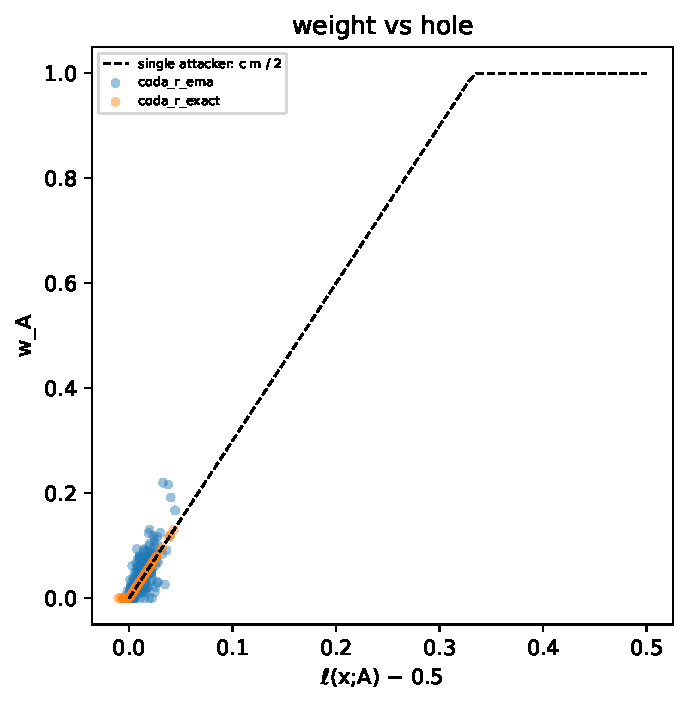
\includegraphics[width=\linewidth]{figures/fig_e2_weight_vs_hole.pdf}
\caption{Scatter of $w_A$ against $\ell(\bx;A)-\tfrac12$ in the controlled vulnerability injection (only rollouts before B is injected). The dashed line is the single-member closed form $\operatorname{clip}(c\mu/2,0,1)$ with $c=6$.}
\label{fig:weight-hole}
\end{minipage}
\end{figure}

\begin{figure}[!htbp]
\begin{center}
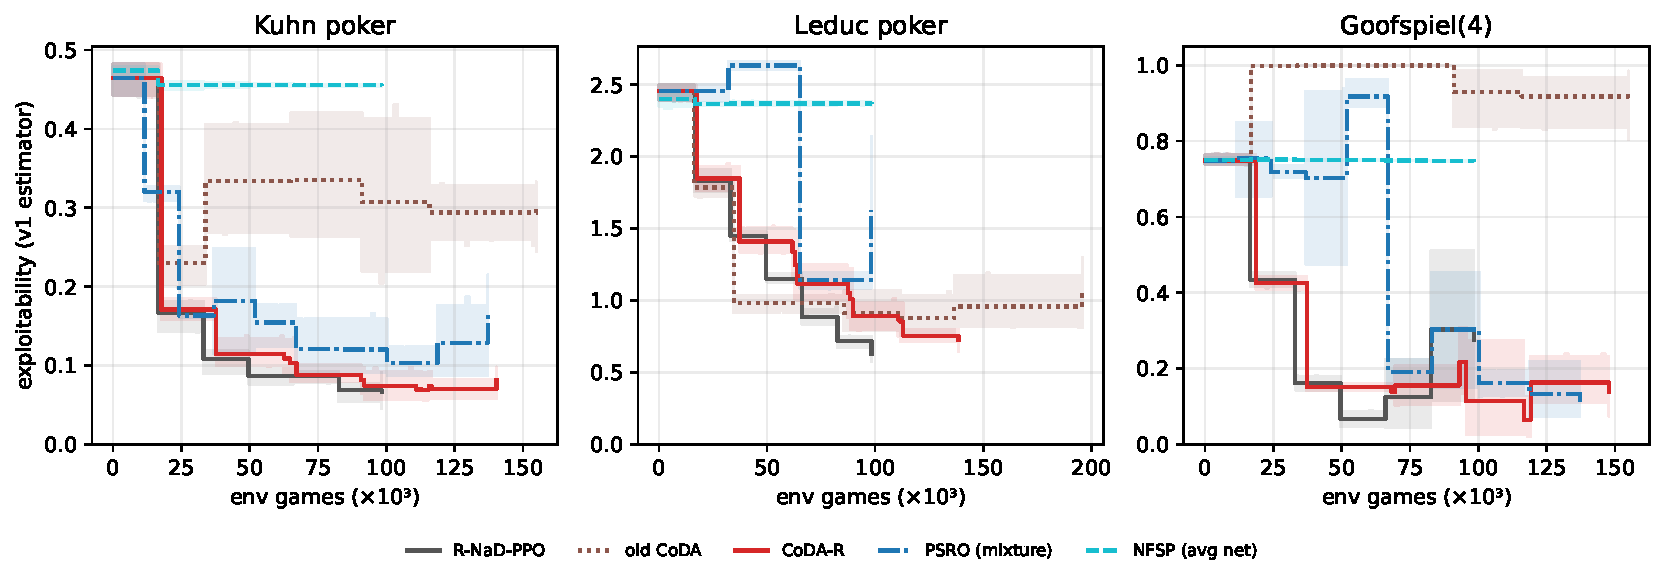
\includegraphics[width=0.9\linewidth]{figures/fig_v1_short_run.pdf}
\end{center}
\caption{Short runs (192 rollouts; the horizontal axis counts all environment games, including diagnostic games; 4 seeds), comparing \codar{}, \rnad{}, \coda{} with a moving dual anchor, the PSRO mixture, and the NFSP average network. Kuhn, \coda{}, and NFSP are reported only here.}
\label{fig:v1}
\end{figure}

\begin{figure}[!htbp]
\centering
\begin{minipage}[b]{0.62\linewidth}
\centering
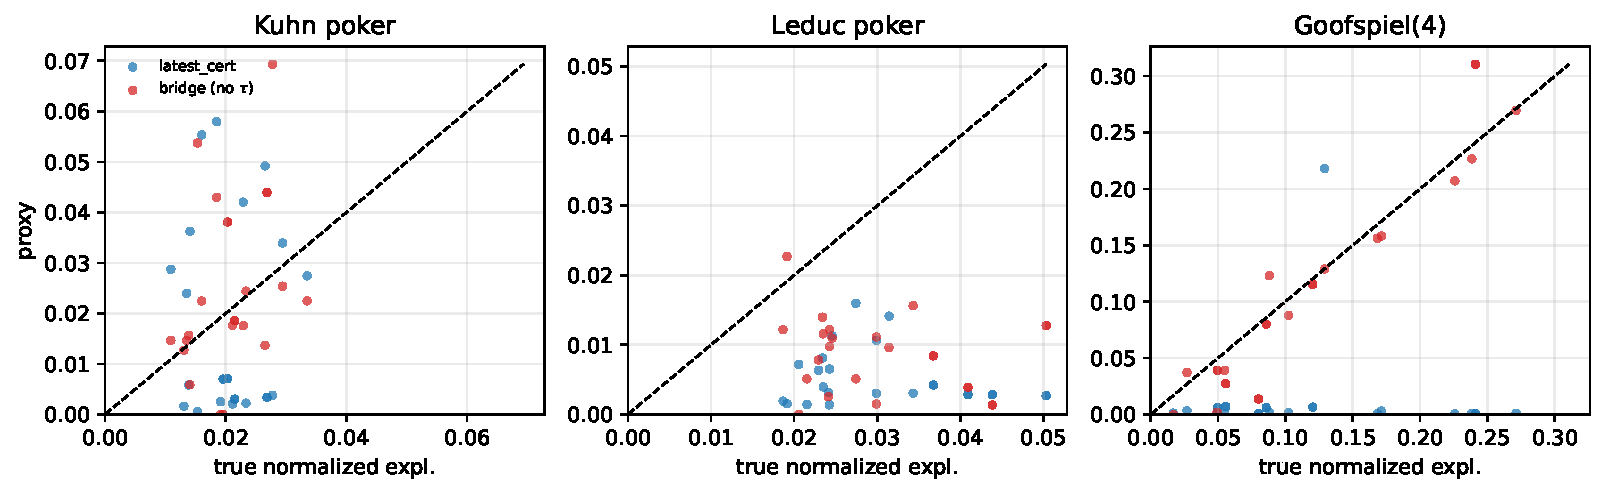
\includegraphics[width=\linewidth]{figures/fig_oracle_bridge.pdf}
\caption{Scatter of two neural proxies against the true normalized exploitability of the same policy at oracle admission times (short runs). \texttt{latest\_cert} falls below the true value 63/72 times, and the bridge proxy 55/72 times.}
\label{fig:bridge}
\end{minipage}\hfill
\begin{minipage}[b]{0.34\linewidth}
\centering
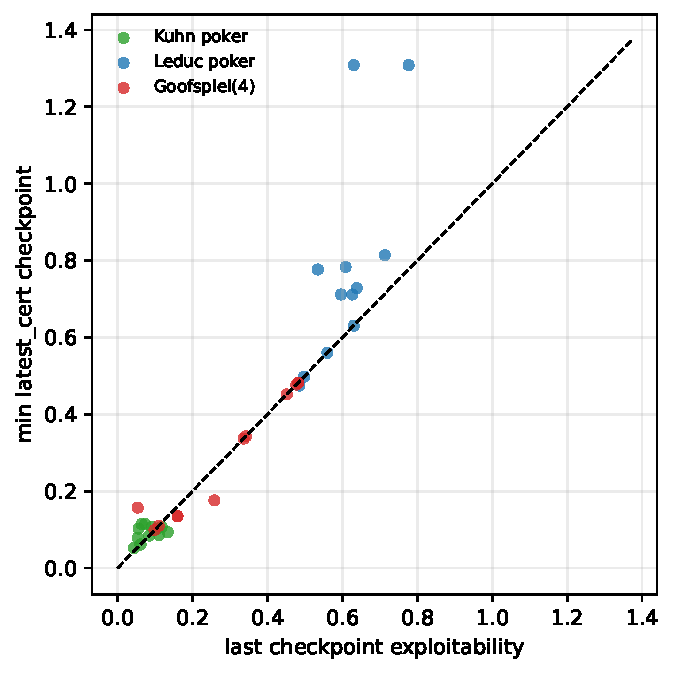
\includegraphics[width=0.8\linewidth]{figures/fig_checkpoint_selection.pdf}
\caption{Checkpoint selection. The horizontal axis is the exploitability of the last checkpoint, and the vertical axis is the exploitability at the minimum of \texttt{latest\_cert}.}
\label{fig:ckpt}
\end{minipage}
\end{figure}

\begin{figure}[!htbp]
\begin{center}
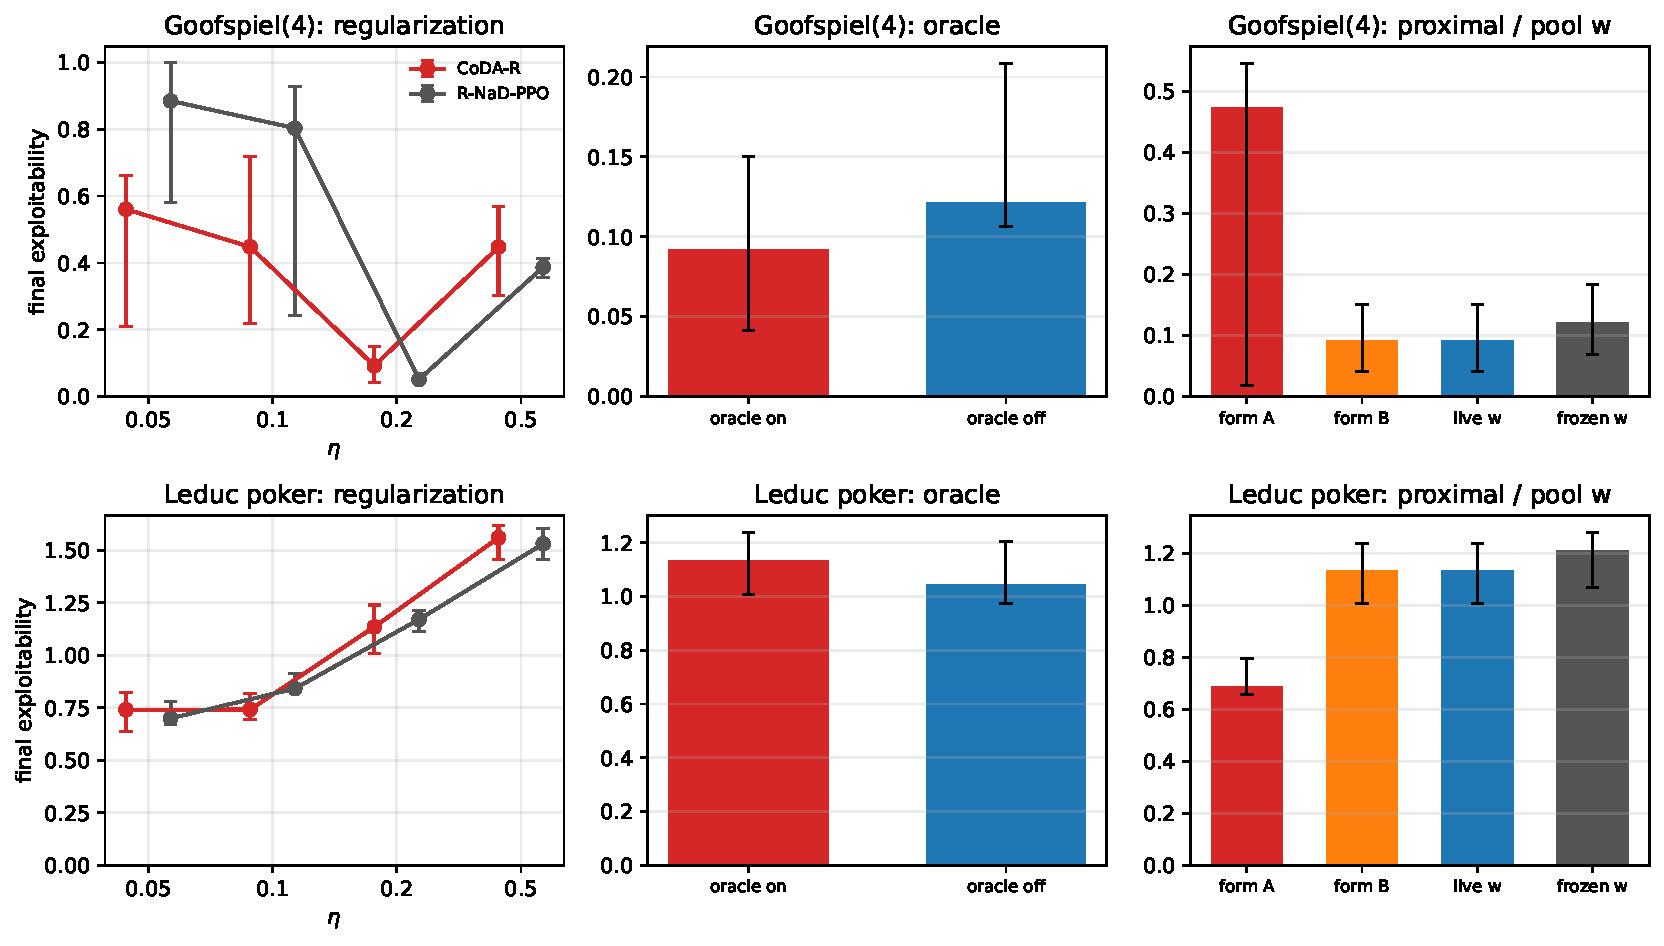
\includegraphics[width=0.85\linewidth]{figures/fig_ablations.pdf}
\end{center}
\caption{Ablations (96 rollouts; final exploitability, IQM $\pm$ CI). Left: $\eta$ grid, shared by \codar{} and \rnad{}. Middle: oracle on/off. Right: proximal-term form A (loss KL) / B (reward shaping), and pool coefficients re-projected every rollout / frozen for a whole period.}
\label{fig:ablations}
\end{figure}

\end{document}
